\chapter{Galerkin 法、配置法及其他方法}\label{ch:5}
\SourcePage{141}

本章简要介绍离散边值问题和初边值问题的几种经典方法.

我们从一个抽象边值问题出发,给出三个简单的例题.把问题改写为弱形式(或变分形式)后,介绍四类不同的空间逼近：Galerkin 法、Petrov--Galerkin 法、配置法和广义 Galerkin 法.对每一类方法,都回顾其主要的稳定性与收敛性质.

随后,讨论初边值问题的时间离散.为此,需要考察时间导数的几个基本有限差分格式,同时说明几种经典的分步法和算子分裂法.

\section{一个用作参照的抽象边值问题}\label{sec:5.1}

照例用 \(\Omega\) 表示 \(\mathbb R^d\) 中的有界区域(\(d=2,3\)),边界为 \(\partial\Omega\).考虑如下形式的边值问题：
\begin{equation}\label{eq:5.1.1}
  \begin{cases}
    Lu=f,&\text{在 }\Omega\text{ 内},\\
    Bu=0,&\text{在 }\partial\Omega^*\text{ 上},
  \end{cases}
\end{equation}
其中 \(f\) 是给定函数,\(u\) 是未知量,\(L\) 是线性微分算子,\(B\) 是仿射边界算子.这里 \(\partial\Omega^*\) 是 \(\partial\Omega\) 的一个子集,也可以是整个边界.通常,\(L\) 是空间 \(H\) 中的无界算子,其中 \(H\) 可以取为 \(L^2(\Omega)\) 或 \(L_w^2(\Omega)\).在 Chebyshev 谱逼近中,后一空间是\eqref{eq:4.5.3}引入的加权 Hilbert 空间.我们在空间 \(X\subset H\) 中寻找解 \(u\),要求 \(L\) 和 \(B\) 对 \(X\) 中的函数有定义.

一般可以把问题\eqref{eq:5.1.1}改写为弱形式(或变分形式).一方面,这种做法允许寻找弱解.弱解不必逐点满足\eqref{eq:5.1.1},这大大拓宽了可处理的物理问题的范围,\SourcePage{142}使数据不光滑的问题也能纳入其中.此外,弱形式便于构造逼近方法,例如 Galerkin 法及其推广,包括 Petrov--Galerkin 法和广义 Galerkin 法等.

在这一阶段,我们在许多地方采用简洁、启发性的论述,因为目的是说明各种方法所依据的基本思想.在后面各章中,会针对不同问题给出精确的数学框架.

形式上,将微分方程乘以适当的试验函数,再在区域上积分,就可以导出弱形式.在这一步,通常用分部积分的 Green 公式
\begin{equation}\label{eq:5.1.2}
  \int_\Omega\frac{\partial u}{\partial x_i}v\,\mathrm d\boldsymbol{x}
  =-\int_\Omega u\frac{\partial v}{\partial x_i}\,\mathrm d\boldsymbol{x}
    +\int_{\partial\Omega}uvn_i\,\mathrm d\gamma,\qquad i=1,\ldots,d,
\end{equation}
以降低对解 \(u\) 的求导阶数.这里 \(\boldsymbol{n}=(n_1,\ldots,n_d)\) 是 \(\partial\Omega\) 上的单位外法向量.

由此得到如下形式的问题：
\begin{equation}\label{eq:5.1.3}
  \text{求 }u\in W,\quad \mathcal A(u,v)=\mathcal F(v)
  \qquad\forall v\in V,
\end{equation}
其中 \(W\) 是容许解的空间,\(V\) 是试验函数空间.可以假定 \(W\) 和 \(V\) 都是 Hilbert 空间.\(\mathcal F\) 是 \(V\) 上的线性泛函,包含右端项 \(f\) 以及可能出现的非齐次边界项.最后,\(\mathcal A(\cdot,\cdot)\) 是与微分算子 \(L\) 相应的双线性形式.

\(u\) 的边界条件可以直接放进 \(W\) 的定义中,这类条件称为\emph{本质边界条件}.也可以通过适当选取双线性形式 \(\mathcal A\) 和泛函 \(\mathcal F\) 间接实现,这类条件称为\emph{自然边界条件}.

在大多数情况下,\(W=V\).无论如何,都要选取适当的空间 \(W\) 和 \(V\),使\eqref{eq:5.1.3}中的所有运算在数学上都有意义.

为了使说明不那么抽象,下面给出三个例题,后文还将详细讨论.这里仍以说明基本思想为主,严格的框架留待后文建立.

\begin{example}[(Poisson 问题)]\label{ex:5.1.1}
问题为
\begin{equation}\label{eq:5.1.4}
  \begin{cases}
    -\Delta u=f,&\text{在 }\Omega\text{ 内},\\
    u=0,&\text{在 }\partial\Omega\text{ 上},
  \end{cases}
\end{equation}
其中 \(f\) 是给定函数,\SourcePage{143}
\[
  \Delta:=\sum_{i=1}^d\frac{\partial^2}{\partial x_i^2}
\]
是 Laplace 算子.这一问题见于许多应用,将在第~\BookRef{ch:6}{6}~章讨论.

为得到其变分形式,回顾 Laplace 算子的 Green 公式：
\begin{equation}\label{eq:5.1.5}
  -\int_\Omega(\Delta u)v\,\mathrm d\boldsymbol{x}
  =\int_\Omega\nabla u\cdot\nabla v\,\mathrm d\boldsymbol{x}
    -\int_{\partial\Omega}\frac{\partial u}{\partial n}v\,\mathrm d\gamma.
\end{equation}
注意到 \(\Delta u=\operatorname{div}\nabla u\),此式可由\eqref{eq:5.1.2}得到.结合\eqref{eq:5.1.4}和\eqref{eq:5.1.5},容易看出 \(u\) 满足形如\eqref{eq:5.1.3}的问题,其中
\begin{equation}\label{eq:5.1.6}
  \begin{cases}
    W=V=H_0^1(\Omega),\\
    \mathcal A(u,v):=\displaystyle\int_\Omega\nabla u\cdot\nabla v\,\mathrm d\boldsymbol{x},\\
    \mathcal F(v):=\displaystyle\int_\Omega fv\,\mathrm d\boldsymbol{x},
  \end{cases}
\end{equation}
而 \(H_0^1(\Omega)\) 在第~\ref{sec:1.2}~节定义.
\end{example}

\begin{example}[(Stokes 问题)]\label{ex:5.1.2}
这一次求解的问题是
\begin{equation}\label{eq:5.1.7}
  \begin{cases}
    -\nu\Delta\boldsymbol{u}+\nabla p=\boldsymbol{f},&\text{在 }\Omega\text{ 内},\\
    \operatorname{div}\boldsymbol{u}=0,&\text{在 }\Omega\text{ 内},\\
    \boldsymbol{u}=\boldsymbol{0},&\text{在 }\partial\Omega\text{ 上},
  \end{cases}
\end{equation}
其中 \(\nu\) 为正常数,\(\boldsymbol{f}\) 是给定的向量函数.第~\BookRef{ch:9}{9}~章讨论这一问题,第~\BookRef{ch:10}{10}~章则在黏性不可压缩流动的 Navier--Stokes 方程框架中推导它.在这里,\(\boldsymbol{u}\) 和 \(p\) 分别表示流体的速度和压力.第一式是线性化的动量方程,第二式表达不可压缩性约束.

问题\eqref{eq:5.1.7}可写成\eqref{eq:5.1.1}的形式,只需令
\[
  u=\begin{pmatrix}\boldsymbol{u}\\p\end{pmatrix},\quad
  f=\begin{pmatrix}\boldsymbol{f}\\0\end{pmatrix},\quad
  L=\begin{pmatrix}-\nu\Delta&\nabla\\\operatorname{div}&0\end{pmatrix},\quad
  B=\begin{pmatrix}I&0\\0&0\end{pmatrix},
\]
其中 \(I\) 是恒等算子.

其变分形式可如下导出.定义
\begin{equation}\label{eq:5.1.8}
  \mathcal V=(H_0^1(\Omega))^d,\qquad
  Q=L_0^2(\Omega):=\left\{q\in L^2(\Omega)\ \middle|\ \int_\Omega q\,\mathrm d\boldsymbol{x}=0\right\}.
\end{equation}
\(\mathcal V\) 是容许速度空间,\(Q\) 是容许压力空间.要求压力平均值为零,是为了使压力唯一.对\eqref{eq:5.1.7}的第一式应用\eqref{eq:5.1.2}和\eqref{eq:5.1.5},得到
\SourcePage{144}
\[
  \nu\int_\Omega\nabla\boldsymbol{u}:\nabla\boldsymbol{v}\,\mathrm d\boldsymbol{x}
  -\int_\Omega p\operatorname{div}\boldsymbol{v}\,\mathrm d\boldsymbol{x}
  =\int_\Omega\boldsymbol{f}\cdot\boldsymbol{v}\,\mathrm d\boldsymbol{x}
  \qquad\forall\boldsymbol{v}\in\mathcal V,
\]
由第二式则得到
\[
  \int_\Omega q\operatorname{div}\boldsymbol{u}\,\mathrm d\boldsymbol{x}=0
  \qquad\forall q\in Q.
\]
因此,令
\begin{equation}\label{eq:5.1.9}
  \left\{
  \begin{aligned}
    W=V&=\mathcal V\times Q,\\
    \mathcal A(u,v)&:=\nu\int_\Omega\nabla\boldsymbol{u}:\nabla\boldsymbol{v}\,\mathrm d\boldsymbol{x}
     -\int_\Omega p\operatorname{div}\boldsymbol{v}\,\mathrm d\boldsymbol{x}
     +\int_\Omega q\operatorname{div}\boldsymbol{u}\,\mathrm d\boldsymbol{x},\\
    \mathcal F(v)&:=\int_\Omega\boldsymbol{f}\cdot\boldsymbol{v}\,\mathrm d\boldsymbol{x},
  \end{aligned}
  \right.
\end{equation}
其中 \(u=(\boldsymbol{u},p)\)、\(v=(\boldsymbol{v},q)\in V\),即可把\eqref{eq:5.1.7}改写为\eqref{eq:5.1.3}.这一推导的更多细节见第~\BookRef{ch:9}{9}~章,不过要注意函数空间的记号有所不同.
\end{example}

\begin{example}[(定常对流问题)]\label{ex:5.1.3}
设 \(\boldsymbol{a}\)、\(a_0\) 和 \(f\) 是 \(\Omega\) 上的给定函数,考虑问题
\begin{equation}\label{eq:5.1.10}
  \begin{cases}
    \boldsymbol{a}\cdot\nabla u+a_0u=f,&\text{在 }\Omega\text{ 内},\\
    u=\varphi,&\text{在 }\partial\Omega^{\mathrm{in}}\text{ 上},
  \end{cases}
\end{equation}
其中
\[
  \partial\Omega^{\mathrm{in}}
  :=\{\boldsymbol{x}\in\partial\Omega\mid\boldsymbol{a}(\boldsymbol{x})\cdot\boldsymbol{n}(\boldsymbol{x})<0\}
\]
称为\emph{流入边界},\(\varphi\) 在其上给定.随 \(\boldsymbol{a}(\boldsymbol{x})\) 取值的不同,\(\partial\Omega^{\mathrm{in}}\) 可以是空集,可以与 \(\partial\Omega\) 一致,也可以是 \(\partial\Omega\) 的真子集.\eqref{eq:5.1.10}的含时版本是流入流出型双曲问题,将在第~\BookRef{ch:14}{14}~章讨论.

\eqref{eq:5.1.10}的一种弱形式可按如下方式得到.按\eqref{eq:5.1.2}分部积分,有
\[
  \begin{aligned}
    \int_\Omega(\boldsymbol{a}\cdot\nabla u)v\,\mathrm d\boldsymbol{x}
    &=-\int_\Omega u\operatorname{div}(\boldsymbol{a}v)\,\mathrm d\boldsymbol{x}
      +\int_{\partial\Omega^{\mathrm{in}}}(\boldsymbol{a}\cdot\boldsymbol{n})\varphi v\,\mathrm d\gamma\\
    &\quad+\int_{\partial\Omega\setminus\partial\Omega^{\mathrm{in}}}
         (\boldsymbol{a}\cdot\boldsymbol{n})uv\,\mathrm d\gamma
         \qquad\forall v\in H^1(\Omega).
  \end{aligned}
\]
注意,边界条件已在分部积分过程中计入.令 \(V=H^1(\Omega)\),并取 \(W\) 为相应的输运图空间,即在 \(L^2(\Omega)\) 中要求 \(\boldsymbol{a}\cdot\nabla u\in L^2(\Omega)\),并具有使流出项有意义的迹.在系数和边界具有相应正则性的条件下,可令
\begin{equation}\label{eq:5.1.11}
  \left\{
  \begin{aligned}
    \mathcal A(u,v)&:=-\int_\Omega u\operatorname{div}(\boldsymbol{a}v)\,\mathrm d\boldsymbol{x}
      +\int_{\partial\Omega\setminus\partial\Omega^{\mathrm{in}}}
           (\boldsymbol{a}\cdot\boldsymbol{n})uv\,\mathrm d\gamma\\
      &\quad+\int_\Omega a_0uv\,\mathrm d\boldsymbol{x},\\
    \mathcal F(v)&:=\int_\Omega fv\,\mathrm d\boldsymbol{x}
      -\int_{\partial\Omega^{\mathrm{in}}}(\boldsymbol{a}\cdot\boldsymbol{n})\varphi v\,\mathrm d\gamma,
  \end{aligned}
  \right.
\end{equation}
从而将\eqref{eq:5.1.10}写成\eqref{eq:5.1.3}的形式.
\end{example}

\subsection{泛函分析的若干结果}\label{sec:5.1.1}
\SourcePage{145}

在考察\eqref{eq:5.1.3}的数值逼近之前,先给出关于解的存在性和唯一性的两个基本泛函分析定理.第一个定理针对 \(W=V\) 这一特殊情形,因而对应于问题
\begin{equation}\label{eq:5.1.12}
  \text{求 }u\in V,\quad \mathcal A(u,v)=\mathcal F(v)
  \qquad\forall v\in V.
\end{equation}

\begin{theorem}[Lax--Milgram 引理]{5.1.1}
设 \(V\) 为实 Hilbert 空间,赋有范数 \(\|\cdot\|\).设 \(\mathcal A\colon V\times V\to\mathbb R\) 是双线性形式,\(\mathcal F\colon V\to\mathbb R\) 是连续线性泛函,即 \(\mathcal F\in V'\),其中 \(V'\) 表示 \(V\) 的对偶空间.进一步假定 \(\mathcal A(\cdot,\cdot)\) 连续,即
\begin{equation}\label{eq:5.1.13}
  \exists\gamma>0:\quad |\mathcal A(w,v)|\le\gamma\|w\|\|v\|
  \qquad\forall w,v\in V,
\end{equation}
且具有强制性,即
\begin{equation}\label{eq:5.1.14}
  \exists\alpha>0:\quad\mathcal A(v,v)\ge\alpha\|v\|^2\qquad\forall v\in V.
\end{equation}
则\eqref{eq:5.1.12}存在唯一解 \(u\in V\),并且
\begin{equation}\label{eq:5.1.15}
  \|u\|\le\frac1\alpha\|\mathcal F\|_{V'}.
\end{equation}
\end{theorem}

\begin{proof}
由 Riesz 表示定理(例如,见\BookCite{yosida1974}{Yosida(1974)}第 90 页),可以写出
\[
  \mathcal F(v)=(R\mathcal F,v)_V\qquad\forall v\in V,
\]
并且对每个固定的 \(w\in V\),
\[
  \mathcal A(w,v)=(Aw,v)_V\qquad\forall v\in V.
\]
这里 \((\cdot,\cdot)_V\) 是 \(V\) 中的内积.双射 \(R\colon V'\to V\) 和 \(A\colon V\to V\) 都是连续线性算子.更确切地说,\(R\) 是等距算子,因为
\[
  \|R\mathcal F\|=\sup_{\substack{v\in V\\v\ne0}}\frac{(R\mathcal F,v)_V}{\|v\|}
     =\sup_{\substack{v\in V\\v\ne0}}\frac{\mathcal F(v)}{\|v\|}
     =\|\mathcal F\|_{V'},
\]
而且由\eqref{eq:5.1.13},
\[
  \|Aw\|=\sup_{\substack{v\in V\\v\ne0}}\frac{(Aw,v)_V}{\|v\|}
     =\sup_{\substack{v\in V\\v\ne0}}\frac{\mathcal A(w,v)}{\|v\|}
     \le\gamma\|w\|.
\]
于是,问题\eqref{eq:5.1.12}等价于：对每个 \(\mathcal F\in V'\),求唯一的 \(u\in V\),使得
\begin{equation}\label{eq:5.1.16}
  Au=R\mathcal F.
\end{equation}
\SourcePage{146}
也就是证明 \(A\) 是双射.

先证明 \(A\) 是单射.我们有
\begin{equation}\label{eq:5.1.17}
  \|v\|^2\le\frac1\alpha(Av,v)_V
    \le\frac1\alpha\|Av\|\|v\|,
\end{equation}
从而 \(\|v\|\le\|Av\|/\alpha\).由此得到唯一性.

现在证明值域 \(\mathcal R(A)\) 是闭的,且 \(\mathcal R(A)^\perp=\{0\}\).这等价于证明 \(\mathcal R(A)=V\).(若 \(S\) 是具有内积 \((\cdot,\cdot)_X\) 的 Hilbert 空间 \(X\) 的闭子空间,则其正交补 \(S^\perp\) 由满足 \((y,x)_X=0\) 对所有 \(x\in S\) 成立的 \(y\in X\) 组成.)设 \(Av_n\to w\) 于 \(V\).由\eqref{eq:5.1.17},
\[
  \|v_n-v_m\|\le\frac1\alpha\|Av_n-Av_m\|,
\]
所以 \(v_n\) 是 Cauchy 序列.设 \(v=\lim_{n\to\infty}v_n\).由 \(A\) 的连续性,\(Av=w\),因此 \(\mathcal R(A)\) 是闭的.取 \(z\in\mathcal R(A)^\perp\),则
\[
  0=(Az,z)_V=\mathcal A(z,z)\ge\alpha\|z\|^2,
\]
即 \(z=0\).

最后只需证明\eqref{eq:5.1.15}.在\eqref{eq:5.1.12}中取 \(v=u\),得到
\[
  \|u\|^2\le\frac1\alpha\mathcal A(u,u)=\frac1\alpha\mathcal F(u)
    \le\frac1\alpha\|\mathcal F\|_{V'}\|u\|,
\]
从而得到\eqref{eq:5.1.15}.\hfill\(\square\)
\end{proof}

\begin{note}\NumberedNote{note:5.1.1}{\heiti(对称情形)}
若双线性形式对称,即
\begin{equation}\label{eq:5.1.18}
  \mathcal A(w,v)=\mathcal A(v,w)\qquad\forall w,v\in V,
\end{equation}
则 \(\mathcal A(\cdot,\cdot)\) 在 \(V\) 上定义一个内积,直接应用 Riesz 表示定理便可推出\eqref{eq:5.1.12}解的存在性和唯一性.再回顾一下,在这种情形下,\eqref{eq:5.1.12}的解可看作下列最小化问题的唯一解：
\begin{equation}\label{eq:5.1.19}
  \text{求 }u\in V,\quad J(u)\le J(v)\qquad\forall v\in V,
\end{equation}
其中
\begin{equation}\label{eq:5.1.20}
  J(v):=\frac12\mathcal A(v,v)-\mathcal F(v)
\end{equation}
是一个二次泛函.\hfill\(\square\)
\end{note}

\begin{note}\NumberedNote{note:5.1.2}{\heiti(复数情形)}
若 \(V\) 是复 Hilbert 空间,就要修改对形式 \(\mathcal A(\cdot,\cdot)\) 的假设.首先,要求 \(\mathcal A\) 是半双线性的,即对第一个变量线性,并且
\[
  \mathcal A(w,c_1v_1+c_2v_2)
   =\overline c_1\mathcal A(w,v_1)+\overline c_2\mathcal A(w,v_2)
\]
\SourcePage{147}
对任意 \(w,v_1,v_2\in V\) 和 \(c_1,c_2\in\mathbb C\) 成立.这里 \(\overline c_k\) 是复数 \(c_k\) 的共轭,\(k=1,2\).相应地,\(\mathcal F\) 为连续共轭线性泛函.此外,强制性假设改为
\begin{equation}\label{eq:5.1.21}
  |\mathcal A(v,v)|\ge\alpha\|v\|^2\qquad\forall v\in V.
\end{equation}
Lax--Milgram 引理的证明基本不变.

在实数情形下,条件\eqref{eq:5.1.21}与\eqref{eq:5.1.14}只差一个整体符号.可以证明,它或者等价于对每个 \(v\in V\) 都有 \(\mathcal A(v,v)\ge\alpha\|v\|^2\),或者等价于对每个 \(v\in V\) 都有 \(-\mathcal A(v,v)\ge\alpha\|v\|^2\).也就是说,\(\mathcal A(\cdot,\cdot)\) 或 \(-\mathcal A(\cdot,\cdot)\) 必须满足\eqref{eq:5.1.14}.\hfill\(\square\)
\end{note}

在 \(W\) 与 \(V\) 不同的更一般情形下,可用下面的结果分析问题\eqref{eq:5.1.3}.这一结果是\BookCite{necas1962}{Nečas(1962)}对 Lax--Milgram 引理的推广.

\begin{theorem}[]{5.1.2}
设 \(W\) 和 \(V\) 是两个实 Hilbert 空间,范数分别为 \(\tnorm{\cdot}\) 和 \(\|\cdot\|\).设存在两个正常数 \(\alpha,\gamma\),使双线性形式 \(\mathcal A\colon W\times V\to\mathbb R\) 满足
\begin{align}
  |\mathcal A(w,v)|&\le\gamma\tnorm{w}\|v\|\qquad\forall w\in W,\ v\in V,
    \label{eq:5.1.22}\\
  \sup_{\substack{v\in V\\v\ne0}}\frac{\mathcal A(w,v)}{\|v\|}
    &\ge\alpha\tnorm{w}\qquad\forall w\in W,
    \label{eq:5.1.23}\\
  \sup_{w\in W}\mathcal A(w,v)&>0\qquad\forall v\in V,\ v\ne0.
    \label{eq:5.1.24}
\end{align}
则对任意 \(\mathcal F\in V'\),\eqref{eq:5.1.3}存在唯一解 \(u\in W\),且
\begin{equation}\label{eq:5.1.25}
  \tnorm{u}\le\frac{\|\mathcal F\|_{V'}}{\alpha}.
\end{equation}
\end{theorem}

\begin{proof}
证明与 Lax--Milgram 引理(定理~\ref{thm:5.1.1})很相似.事实上,由 Riesz 表示定理,可构造连续线性算子 \(A\colon W\to V\),使得
\begin{equation}\label{eq:5.1.26}
  \mathcal A(w,v)=(Aw,v)_V\qquad\forall v\in V
\end{equation}
对每个 \(w\in W\) 成立,其中 \((\cdot,\cdot)_V\) 表示 \(V\) 中的内积.此外,
\[
  \|Aw\|\le\gamma\tnorm{w}\qquad\forall w\in W.
\]
于是问题归结为：对任意给定的 \(\mathcal F\in V'\),求唯一的 \(u\in W\),使得
\begin{equation}\label{eq:5.1.27}
  Au=R\mathcal F.
\end{equation}
这里 \(R\colon V'\to V\) 是定理~\ref{thm:5.1.1}的证明中构造的等距算子.

\SourcePage{148}
由\eqref{eq:5.1.23}和\eqref{eq:5.1.26}立即可知,\(Aw=0\) 蕴含 \(w=0\),即 \(A\) 是单射.

此外,\(A\) 的值域 \(\mathcal R(A)\) 是闭的.事实上,若 \(Aw_n\to v\) 于 \(V\),则
\[
  \tnorm{w_n-w_m}\le\frac1\alpha
    \sup_{\substack{v_0\in V\\v_0\ne0}}
        \frac{\mathcal A(w_n-w_m,v_0)}{\|v_0\|}
    \le\frac1\alpha\|A(w_n-w_m)\|,
\]
所以 \(w_n\to w\) 于 \(W\),且 \(Aw_n\to Aw=v\) 于 \(V\).最后,若 \(z\in\mathcal R(A)^\perp\),即
\[
  (Aw,z)_V=\mathcal A(w,z)=0\qquad\forall w\in W,
\]
则由\eqref{eq:5.1.24}可知 \(z=0\),故 \(A\) 是满射.这样就证明了,对每个 \(\mathcal F\in V'\),\eqref{eq:5.1.27}存在唯一解 \(u\).

此外,
\[
  \alpha\tnorm{u}\le\sup_{\substack{v\in V\\v\ne0}}\frac{(Au,v)_V}{\|v\|}
    =\sup_{\substack{v\in V\\v\ne0}}\frac{(R\mathcal F,v)_V}{\|v\|}
    =\|\mathcal F\|_{V'},
\]
所以\eqref{eq:5.1.25}成立.\hfill\(\square\)
\end{proof}

\section{Galerkin 法}\label{sec:5.2}

现在考虑 \(W=V\) 的情形,因此所讨论的问题是\eqref{eq:5.1.12}.

设 \(h>0\) 是一个在应用中将取“小值”的参数.在有限元法中,\(h\) 是网格间距；在谱方法中,它是谱解的多项式次数的倒数,见第~\ref{ch:3}~章和第~\ref{ch:4}~章.记
\begin{equation}\label{eq:5.2.1}
  \{V_h\mid h>0\}
\end{equation}
为 \(V\) 的一族有限维子空间.假设
\begin{equation}\label{eq:5.2.2}
  \forall v\in V,\qquad
  \inf_{v_h\in V_h}\|v-v_h\|\longrightarrow0
  \quad\text{当 }h\to0\text{ 时.}
\end{equation}
\eqref{eq:5.1.12}的 Galerkin 逼近如下.给定 \(\mathcal F\in V'\),
\begin{equation}\label{eq:5.2.3}
  \text{求 }u_h\in V_h,\quad \mathcal A(u_h,v_h)=\mathcal F(v_h)
  \qquad\forall v_h\in V_h.
\end{equation}
因此,这是一种对\eqref{eq:5.1.12}的\emph{内部逼近}.从代数的角度看,设 \(\{\varphi_j\mid j=1,\ldots,N_h\}\) 是向量空间 \(V_h\) 的一组基,可以写成
\begin{equation}\label{eq:5.2.4}
  u_h(\boldsymbol{x})=\sum_{j=1}^{N_h}\xi_j\varphi_j(\boldsymbol{x}).
\end{equation}
\SourcePage{149}
由\eqref{eq:5.2.3}得到下列 \(N_h\) 阶线性方程组：
\begin{equation}\label{eq:5.2.5}
  A\boldsymbol{\xi}=\boldsymbol{F},
\end{equation}
其中 \(\boldsymbol{\xi}=(\xi_j)\)、\(\boldsymbol{F}:=(\mathcal F(\varphi_i))\),而 \(A_{ij}:=\mathcal A(\varphi_j,\varphi_i)\)(\(i,j=1,\ldots,N_h\)).矩阵 \(A\) 称为\emph{刚度矩阵}.它的性质见后面的笔记~\ref{note:5.2.2}.

对于问题\eqref{eq:5.2.3},有下列结果.

\begin{theorem}[]{5.2.1}
在定理~\ref{thm:5.1.1}的假设下,\eqref{eq:5.2.3}有唯一解 \(u_h\),而且这个解是稳定的,因为
\begin{equation}\label{eq:5.2.6}
  \|u_h\|\le\frac{\|\mathcal F\|_{V'}}{\alpha}.
\end{equation}
此外,若 \(u\) 是\eqref{eq:5.1.12}的解,则
\begin{equation}\label{eq:5.2.7}
  \|u-u_h\|\le\frac\gamma\alpha\inf_{v_h\in V_h}\|u-v_h\|.
\end{equation}
由\eqref{eq:5.2.2}可知 \(u_h\) 收敛到 \(u\).
\end{theorem}

\begin{proof}
由于 \(V_h\) 是 \(V\) 的子空间,在假设\eqref{eq:5.1.13}和\eqref{eq:5.1.14}下,可以对问题\eqref{eq:5.2.3}应用 Lax--Milgram 引理,得到 \(u_h\) 的存在性和唯一性.取 \(v_h=u_h\),由\eqref{eq:5.1.14}可得
\[
  \alpha\|u_h\|^2\le\mathcal A(u_h,u_h)=\mathcal F(u_h)
    \le\|\mathcal F\|_{V'}\|u_h\|.
\]
于是得到\eqref{eq:5.2.6}.由于 \(\|\mathcal F\|_{V'}\) 和 \(\alpha\) 都与 \(h\) 无关,这便给出了稳定性.现在将\eqref{eq:5.1.12}的试验函数限制在 \(V_h\) 中,再减去\eqref{eq:5.2.3},得到
\begin{equation}\label{eq:5.2.8}
  \mathcal A(u-u_h,v_h)=0\qquad\forall v_h\in V_h.
\end{equation}
利用\eqref{eq:5.1.13}、\eqref{eq:5.1.14},并在\eqref{eq:5.2.8}中取 \(v_h=w_h-u_h\),其中 \(w_h\in V_h\),可得
\[
  \begin{aligned}
    \alpha\|u-u_h\|^2
    &\le\mathcal A(u-u_h,u-u_h)=\mathcal A(u-u_h,u-w_h)\\
    &\le\gamma\|u-u_h\|\|u-w_h\|\qquad\forall w_h\in V_h.
  \end{aligned}
\]
由此得到\eqref{eq:5.2.7}.\hfill\(\square\)
\end{proof}

估计\eqref{eq:5.2.7}通常称为 Céa 引理.

\begin{note}\NumberedNote{note:5.2.1}{\heiti(对称情形)}
当 \(\mathcal A(\cdot,\cdot)\) 对称时,Galerkin 法称为 Ritz 法.这时,\eqref{eq:5.2.3}解的存在性和唯一性仍可由 Riesz 表示定理推出.此外,\eqref{eq:5.2.8}表明,在 \(\mathcal A\) 诱导的内积下,误差 \(u-u_h\) 与 \(V_h\) 正交.因此,\(u_h\) 是\SourcePage{150}\(u\) 关于同一内积到 \(V_h\) 的正交投影,可立即得到不等式\eqref{eq:5.2.7},而且其中的常数可改进为 \((\gamma/\alpha)^{1/2}\).\hfill\(\square\)
\end{note}

\begin{note}\NumberedNote{note:5.2.2}{\heiti(刚度矩阵 \(A\) 的性质)}
\eqref{eq:5.2.5}中定义的矩阵 \(A\) 是正定的,即对任意非零向量 \(\boldsymbol{\eta}\in\mathbb R^{N_h}\),均有 \((A\boldsymbol{\eta},\boldsymbol{\eta})>0\),其中 \((\cdot,\cdot)\) 表示 Euclid 内积.事实上,令 \(\eta_h\in V_h\) 为函数
\begin{equation}\label{eq:5.2.9}
  \eta_h(\boldsymbol{x})=\sum_{j=1}^{N_h}\eta_j\varphi_j(\boldsymbol{x}).
\end{equation}
则
\[
  (A\boldsymbol{\eta},\boldsymbol{\eta})
   =\sum_{i,j=1}^{N_h}\eta_i\mathcal A(\varphi_j,\varphi_i)\eta_j
   =\mathcal A(\eta_h,\eta_h),
\]
由\eqref{eq:5.1.14}即得结论.特别地,\(A\) 的每个特征值都具有正实部.

因此,\eqref{eq:5.2.3}解的存在性和唯一性也可以用纯代数论证证明,无需诉诸 Lax--Milgram 引理.

当双线性形式 \(\mathcal A\) 对称时,立即可知 \(A\) 也对称.\hfill\(\square\)
\end{note}

\section{Petrov--Galerkin 法}\label{sec:5.3}

这里的数值问题为
\begin{equation}\label{eq:5.3.1}
  \text{求 }u_h\in W_h,\quad
  \mathcal A_h(u_h,v_h)=\mathcal F_h(v_h)\qquad\forall v_h\in V_h,
\end{equation}
其中 \(\{W_h\mid h>0\}\) 和 \(\{V_h\mid h>0\}\) 是两族有限维空间.对每个 \(h>0\),\(W_h\ne V_h\),但 \(\dim W_h=\dim V_h=N_h\).

如果 \(\mathcal A_h\colon W_h\times V_h\to\mathbb R\) 和 \(\mathcal F_h\colon V_h\to\mathbb R\) 分别是 \(\mathcal A\) 和 \(\mathcal F\) 的适当逼近(也可与它们一致),且 \(W_h\) 是 \(W\) 的子空间,\(V_h\) 是 \(V\) 的子空间,那么可以把\eqref{eq:5.3.1}看作\eqref{eq:5.1.3}的逼近.这里,\(W\) 与 \(V\) 可以是同一个空间.

\eqref{eq:5.3.1}的代数表述如下.令 \(\{\varphi_j\mid j=1,\ldots,N_h\}\) 是 \(W_h\) 的一组基,\(\{\psi_i\mid i=1,\ldots,N_h\}\) 是 \(V_h\) 的一组基.仍按\eqref{eq:5.2.4}展开\eqref{eq:5.3.1}的解 \(u_h\),便得到下列 \(N_h\) 阶方程组：
\begin{equation}\label{eq:5.3.2}
  A\boldsymbol{\xi}=\boldsymbol{F},
\end{equation}
其中 \(\boldsymbol{\xi}=(\xi_j)\)、\(\boldsymbol{F}:=(\mathcal F_h(\psi_i))\),\(A_{ij}:=\mathcal A_h(\varphi_j,\psi_i)\).

\SourcePage{151}
对于\eqref{eq:5.3.1}的稳定性和收敛性分析,有如下由 Babuška 得到的定理(例如,见\BookCite{babuska-aziz1972}{Babuška 和 Aziz(1972)}).

\begin{theorem}[]{5.3.1}
在定理~\ref{thm:5.1.2}的假设下,再设 \(\mathcal F_h\colon V_h\to\mathbb R\) 是线性映射,\(\mathcal A_h\colon W_h\times V_h\to\mathbb R\) 是双线性形式,满足与 \(\mathcal A\) 的条件\eqref{eq:5.1.23}、\eqref{eq:5.1.24}相同的性质,其中用 \(W_h\) 代替 \(W\),用 \(V_h\) 代替 \(V\),用 \(\alpha_h\) 代替 \(\alpha\).则\eqref{eq:5.3.1}存在唯一解 \(u_h\),且
\begin{equation}\label{eq:5.3.3}
  \tnorm{u_h}\le\frac1{\alpha_h}
    \sup_{\substack{v_h\in V_h\\v_h\ne0}}\frac{\mathcal F_h(v_h)}{\|v_h\|}.
\end{equation}
进一步,若 \(u\) 是\eqref{eq:5.1.3}的解,则
\begin{equation}\label{eq:5.3.4}
  \begin{aligned}
    \tnorm{u-u_h}\le{}&
      \inf_{w_h\in W_h}\left[\left(1+\frac\gamma{\alpha_h}\right)\tnorm{u-w_h}
       +\frac1{\alpha_h}\sup_{\substack{v_h\in V_h\\v_h\ne0}}
         \frac{|\mathcal A(w_h,v_h)-\mathcal A_h(w_h,v_h)|}{\|v_h\|}\right]\\
     &+\frac1{\alpha_h}\sup_{\substack{v_h\in V_h\\v_h\ne0}}
             \frac{|\mathcal F(v_h)-\mathcal F_h(v_h)|}{\|v_h\|}.
  \end{aligned}
\end{equation}
\end{theorem}

\begin{proof}
对任意固定的 \(h\),存在性和唯一性由定理~\ref{thm:5.1.2}推出.此外,将\eqref{eq:5.1.23}用于 \(\mathcal A_h\) 的对应条件,并用\eqref{eq:5.3.1},得到\eqref{eq:5.3.3}.事实上,
\[
  \tnorm{u_h}\le\frac1{\alpha_h}\sup_{\substack{v_h\in V_h\\v_h\ne0}}
       \frac{\mathcal A_h(u_h,v_h)}{\|v_h\|}
    =\frac1{\alpha_h}\sup_{\substack{v_h\in V_h\\v_h\ne0}}
       \frac{\mathcal F_h(v_h)}{\|v_h\|}.
\]
为证明\eqref{eq:5.3.4},注意对所有 \(w_h\in W_h\) 和 \(v_h\in V_h\),有
\[
  \begin{aligned}
    \mathcal A_h(u_h-w_h,v_h)
     &=\mathcal A(u-w_h,v_h)+\mathcal A(w_h,v_h)-\mathcal A_h(w_h,v_h)\\
     &\quad+\mathcal F_h(v_h)-\mathcal F(v_h).
  \end{aligned}
\]
利用\eqref{eq:5.1.22}以及\eqref{eq:5.1.23}的离散对应式,得到
\[
  \begin{aligned}
    \alpha_h\tnorm{u_h-w_h}\le{}&\gamma\tnorm{u-w_h}\\
      &+\sup_{\substack{v_h\in V_h\\v_h\ne0}}\left\{
         \frac{|\mathcal A(w_h,v_h)-\mathcal A_h(w_h,v_h)|}{\|v_h\|}
         +\frac{|\mathcal F(v_h)-\mathcal F_h(v_h)|}{\|v_h\|}\right\}.
  \end{aligned}
\]
再用三角不等式
\[
  \tnorm{u-u_h}\le\tnorm{u-w_h}+\tnorm{u_h-w_h},
\]
便得到\eqref{eq:5.3.4}.\hfill\(\square\)
\end{proof}

\SourcePage{152}
Petrov--Galerkin 逼近的例子有通常所说的 \(\tau\) 法(例如,见\BookCite{canuto-hussaini-quarteroni-zang1988}{Canuto、Hussaini、Quarteroni 和 Zang(1988)}第 10.4 节),以及对流--扩散方程的迎风处理(见第~\BookRef{sec:8.2.2}{8.2.2}~节).

此外,Petrov--Galerkin 逼近有时可写成
\begin{equation}\label{eq:5.3.5}
  \text{求 }u_h\in W_h,\quad
  \mathcal A_h(u_h,w_h+L_hw_h)=\mathcal F_h(w_h+L_hw_h)
    \qquad\forall w_h\in W_h,
\end{equation}
其中 \(L_h\) 是按某种准则选择的、与 \(L\) 有关的适当算子.令
\[
  V_h:=\{w_h+L_hw_h\mid w_h\in W_h\},
\]
即可将问题\eqref{eq:5.3.5}写成\eqref{eq:5.3.1}的形式.在第~\BookRef{sec:14.3}{14.3}~节可以找到这类例子,其中用 GALS、SUPG 和 DWG 法逼近纯对流方程(见笔记~\BookRef{note:14.3.1}{14.3.1}).

\section{配置法}\label{sec:5.4}

配置法用于几种有限维逼近,尤其见于边界元法、有限元法和谱方法.为简明起见,这里只讨论最后一种情形,因为配置法在谱方法中的应用远比其他情形成功.

因此,可以将讨论限于区域 \(\Omega=(-1,1)^d\),\(d=2,3\),并假设所求离散解是一个关于每个坐标的次数均不超过 \(N\) 的代数多项式.此外,给定 \((N+1)^d\) 个配置点 \(\boldsymbol{x}_i\in\overline\Omega\),它们是 Gauss--Lobatto 求积公式的节点(见\eqref{eq:4.5.19}或\eqref{eq:4.5.38}).

谱配置解是一个函数 \(u_N\in\mathbb Q_N\),其中 \(\mathbb Q_N\) 是关于每个变量 \(x_i\)(\(i=1,\ldots,d\))的次数分别不超过 \(N\) 的代数多项式空间.它满足
\begin{equation}\label{eq:5.4.1}
  \begin{cases}
    L_Nu_N=f,&\text{在节点 }\boldsymbol{x}_i\in\overline\Omega\setminus\partial\Omega^*\text{ 处},\\
    B_Nu_N=0,&\text{在节点 }\boldsymbol{x}_i\in\partial\Omega^*\text{ 处},
  \end{cases}
\end{equation}
其中通常用 \(L_N\) 逼近 \(L\),做法是将各导数替换为伪谱导数,也就是在节点 \(\{\boldsymbol{x}_i\}\) 上插值得到的多项式的精确导数(见第~\ref{sec:4.3.2}~节和第~\ref{sec:4.4.2}~节).\(B_N\) 也作相应处理.

这样,就在 \(\partial\Omega^*\) 上的所有节点处施加边界条件,并在其余所有 Gauss--Lobatto 节点处施加微分方程.更确切地说,若 \(Bu=0\) 表示\SourcePage{153}自然边界条件,也可在 \(\partial\Omega^*\) 的节点处施加该边界条件与微分方程残差的适当线性组合.这样便在离散层面以自然方式施加边界条件.

我们将在第~\BookRef{sec:6.2.2}{6.2.2}~节看到,当原问题具有\eqref{eq:5.1.12}的形式时,这一做法归结为求解
\begin{equation}\label{eq:5.4.2}
  \text{求 }u_N\in V_N,\quad
   \mathcal A_N(u_N,v_N)=\mathcal F_N(v_N)\qquad\forall v_N\in V_N,
\end{equation}
其中 \(V_N=\mathbb Q_N\cap V\),而 \(\mathcal A_N\) 是对形式 \(\mathcal A\) 的逼近,其中所有积分均通过 Gauss--Lobatto 求积公式计算.右端项作同样的逼近.

\eqref{eq:5.4.2}称为谱配置法的\emph{弱形式},而\eqref{eq:5.4.1}称为\emph{强形式}.写成\eqref{eq:5.4.2}时,这一问题实际上表现为广义 Galerkin 法,因此适用下一节的稳定性和收敛性分析.

从代数的角度看,令 \(\{\psi_j\}\) 表示强形式中 \(\mathbb Q_N\) 的 Lagrange 基,即
\begin{equation}\label{eq:5.4.3}
  \psi_j\in\mathbb Q_N,\qquad \psi_j(\boldsymbol{x}_i)=\delta_{ij}
    \qquad\forall i,j=1,\ldots,(N+1)^d.
\end{equation}
令
\[
  u_N(\boldsymbol{x})=\sum_j\xi_j\psi_j(\boldsymbol{x}),\qquad
  \xi_j=u_N(\boldsymbol{x}_j),
\]
由\eqref{eq:5.4.1}可得
\begin{equation}\label{eq:5.4.4}
  \begin{cases}
    \displaystyle\sum_j(L_N\psi_j)(\boldsymbol{x}_i)\xi_j=f(\boldsymbol{x}_i),
        &\text{对所有使 \(\boldsymbol{x}_i\in\overline\Omega\setminus\partial\Omega^*\) 的 \(i\)},\\[3pt]
    \displaystyle\sum_j(B_N^{\mathrm{lin}}\psi_j)(\boldsymbol{x}_i)\xi_j
         =-(B_N0)(\boldsymbol{x}_i),
        &\text{对所有使 \(\boldsymbol{x}_i\in\partial\Omega^*\) 的 \(i\)},
  \end{cases}
\end{equation}
其中 \(B_N^{\mathrm{lin}}v:=B_Nv-B_N0\) 是仿射算子 \(B_N\) 的线性部分.若边界条件齐次,第二式右端为零.这就得到了关于 \(\boldsymbol{\xi}=(\xi_j)\) 的线性方程组,其矩阵可以用伪谱微分矩阵表示.因此,谱配置法也称为\emph{伪谱法}.

\section{广义 Galerkin 法}\label{sec:5.5}

在这种情形下,有限维问题为
\begin{equation}\label{eq:5.5.1}
  \text{求 }u_h\in V_h,\quad
  \mathcal A_h(u_h,v_h)=\mathcal F_h(v_h)\qquad\forall v_h\in V_h,
\end{equation}
其中 \(\{V_h\mid h>0\}\) 是 \(V\) 的一族有限维子空间.\(\mathcal A_h\) 和 \(\mathcal F_h\) 分别表示 \(\mathcal A\) 和 \(\mathcal F\) 的适当逼近.这是\eqref{eq:5.3.1}在允许试探空间与试验空间相同时的情形,包括配置法的\SourcePage{154}弱形式\eqref{eq:5.4.2}.不过,这里单独给出分析,因为本情形的收敛性证明有些不同.广义 Galerkin 法的其他例子包括使用数值积分的 Galerkin 有限元法(见第~\BookRef{sec:6.2.3}{6.2.3}~节),以及对流--扩散问题和 Stokes 问题的稳定化方法(见第~\BookRef{sec:8.3}{8.3}~节和第~\BookRef{sec:9.4}{9.4}~节).

回顾一下,\(\mathcal F_h(\cdot)\) 是定义在 \(V_h\) 上的线性泛函,\(\mathcal A_h(\cdot,\cdot)\) 是定义在 \(V_h\times V_h\) 上的双线性形式.将它们作用于 \(V\) 的元素时,未必有意义.事实上,\(\mathcal A_h\) 和 \(\mathcal F_h\) 往往涉及 \(u_h\) 或其导数的点值,而 \(V\) 中函数未必有这样的点值.例如,上面讨论的三个例题就都无法保证所需的点值有定义.

下述结果称为 Strang 第一引理.

\begin{theorem}[]{5.5.1}
在定理~\ref{thm:5.1.1}的假设下,再设 \(\mathcal F_h(\cdot)\) 是线性映射,双线性形式 \(\mathcal A_h(\cdot,\cdot)\) 在 \(V_h\times V_h\) 上一致强制.这意味着存在 \(\alpha^*>0\),使得对所有 \(h>0\),
\begin{equation}\label{eq:5.5.2}
  \mathcal A_h(v_h,v_h)\ge\alpha^*\|v_h\|^2\qquad\forall v_h\in V_h.
\end{equation}
则\eqref{eq:5.5.1}存在唯一解 \(u_h\),且
\begin{equation}\label{eq:5.5.3}
  \|u_h\|\le\frac1{\alpha^*}\sup_{\substack{v_h\in V_h\\v_h\ne0}}
                \frac{\mathcal F_h(v_h)}{\|v_h\|}.
\end{equation}
若 \(u\) 是\eqref{eq:5.1.12}的解,则
\begin{equation}\label{eq:5.5.4}
  \begin{aligned}
    \|u-u_h\|\le{}&
      \inf_{w_h\in V_h}\left[\left(1+\frac\gamma{\alpha^*}\right)\|u-w_h\|
        +\frac1{\alpha^*}\sup_{\substack{v_h\in V_h\\v_h\ne0}}
           \frac{|\mathcal A(w_h,v_h)-\mathcal A_h(w_h,v_h)|}{\|v_h\|}\right]\\
    &+\frac1{\alpha^*}\sup_{\substack{v_h\in V_h\\v_h\ne0}}
          \frac{|\mathcal F(v_h)-\mathcal F_h(v_h)|}{\|v_h\|}.
  \end{aligned}
\end{equation}
\end{theorem}

\begin{proof}
与定理~\ref{thm:5.3.1}的证明类似,由于\eqref{eq:5.5.2}成立,Lax--Milgram 引理给出存在性、唯一性和不等式\eqref{eq:5.5.3}.虽然\eqref{eq:5.5.4}的证明与\eqref{eq:5.3.4}的证明相差不大,为便于阅读,仍写在下面.

取 \(V_h\) 中任意元素 \(w_h\),令 \(\sigma_h:=u_h-w_h\).由\eqref{eq:5.5.2},
\[
  \begin{aligned}
    \alpha^*\|\sigma_h\|^2&\le\mathcal A_h(\sigma_h,\sigma_h)\\
      &=\mathcal A(u-w_h,\sigma_h)+\mathcal A(w_h,\sigma_h)
         -\mathcal A_h(w_h,\sigma_h)+\mathcal F_h(\sigma_h)-\mathcal F(\sigma_h).
  \end{aligned}
\]
\SourcePage{155}
设 \(\sigma_h\ne0\).由\eqref{eq:5.1.13},
\[
  \begin{aligned}
    \alpha^*\|\sigma_h\|
    &\le\gamma\|u-w_h\|
      +\frac{|\mathcal A(w_h,\sigma_h)-\mathcal A_h(w_h,\sigma_h)|}{\|\sigma_h\|}
      +\frac{|\mathcal F_h(\sigma_h)-\mathcal F(\sigma_h)|}{\|\sigma_h\|}\\
    &\le\gamma\|u-w_h\|+
       \sup_{\substack{v_h\in V_h\\v_h\ne0}}
          \frac{|\mathcal A(w_h,v_h)-\mathcal A_h(w_h,v_h)|}{\|v_h\|}\\
    &\quad+\sup_{\substack{v_h\in V_h\\v_h\ne0}}
        \frac{|\mathcal F_h(v_h)-\mathcal F(v_h)|}{\|v_h\|}.
  \end{aligned}
\]
当 \(\sigma_h=0\) 时,最后的不等式显然也成立.将它与三角不等式
\(\|u-u_h\|\le\|u-w_h\|+\|\sigma_h\|\) 结合,再对 \(w_h\in V_h\) 取下确界,就得到所需结果.\hfill\(\square\)
\end{proof}

下列结果也很有用.

\begin{proposition}[]{5.5.1}
在定理~\ref{thm:5.5.1}的假设下,再设双线性形式 \(\mathcal A_h(\cdot,\cdot)\) 在 \((u,v_h)\) 上有定义,其中 \(u\) 是\eqref{eq:5.1.12}的解,\(v_h\in V_h\).并且,对某个适当的 \(\gamma^*>0\),
\begin{equation}\label{eq:5.5.5}
  |\mathcal A_h(u-w_h,v_h)|\le\gamma^*\|u-w_h\|\|v_h\|
    \qquad\forall w_h,v_h\in V_h,
\end{equation}
此估计对 \(h>0\) 一致成立.则有如下收敛估计：
\begin{equation}\label{eq:5.5.6}
  \begin{aligned}
    \|u-u_h\|\le{}&\left(1+\frac{\gamma^*}{\alpha^*}\right)
                    \inf_{w_h\in V_h}\|u-w_h\|\\
      &+\frac1{\alpha^*}\sup_{\substack{v_h\in V_h\\v_h\ne0}}
          \frac{|\mathcal A_h(u,v_h)-\mathcal F_h(v_h)|}{\|v_h\|}.
  \end{aligned}
\end{equation}
\end{proposition}

\begin{proof}
设 \(w_h\) 是 \(V_h\) 中的任意元素.可以写成
\[
  \begin{aligned}
    \mathcal A_h(u_h-w_h,u_h-w_h)
    &=\mathcal A_h(u-w_h,u_h-w_h)\\
    &\quad+\mathcal F_h(u_h-w_h)-\mathcal A_h(u,u_h-w_h).
  \end{aligned}
\]
由\eqref{eq:5.5.2}和\eqref{eq:5.5.5}得到
\[
  \|u_h-w_h\|\le\frac{\gamma^*}{\alpha^*}\|u-w_h\|
    +\frac1{\alpha^*}\sup_{\substack{v_h\in V_h\\v_h\ne0}}
        \frac{|\mathcal F_h(v_h)-\mathcal A_h(u,v_h)|}{\|v_h\|}.
\]
由三角不等式立即得到\eqref{eq:5.5.6}.\hfill\(\square\)
\end{proof}

从代数的角度看,若按\eqref{eq:5.2.4}展开 \(u_h\),则问题\eqref{eq:5.5.1}给出一个形如\eqref{eq:5.2.5}的线性方程组,其中 \(\mathcal F(\cdot)\) 和 \(\mathcal A(\cdot,\cdot)\) \SourcePage{156}分别换成 \(\mathcal F_h(\cdot)\) 和 \(\mathcal A_h(\cdot,\cdot)\).强制性假设\eqref{eq:5.5.2}保证 \(A\) 是正定矩阵.若 \(\mathcal A_h(\cdot,\cdot)\) 是对称形式,则 \(A\) 也对称.

\begin{note}\NumberedNote{note:5.5.1}{\heiti(非协调逼近)}
\eqref{eq:5.5.1}的一个特殊情形是 \(V_h\) 并非 \(V\) 的子空间,因而双线性形式 \(\mathcal A\) 未必在 \(V_h\times V_h\) 上有定义.假设在 \(V+V_h\) 上定义了范数 \(\|\cdot\|_h\) 和近似双线性形式 \(\mathcal A_h(\cdot,\cdot)\),并在 \(V_h\) 上定义了近似线性泛函 \(\mathcal F_h(\cdot)\).进一步要求存在常数 \(\alpha^*,\gamma^*>0\),使得对每个 \(h>0\),
\[
  \begin{aligned}
    \mathcal A_h(v_h,v_h)&\ge\alpha^*\|v_h\|_h^2
      &&\forall v_h\in V_h,\\
    |\mathcal A_h(w,v_h)|&\le\gamma^*\|w\|_h\|v_h\|_h
      &&\forall w\in V+V_h,\quad v_h\in V_h.
  \end{aligned}
\]
由所谓的 Strang 第二引理,得到下列误差估计：
\[
  \|u-u_h\|_h\le
     \left(1+\frac{\gamma^*}{\alpha^*}\right)\inf_{w_h\in V_h}\|u-w_h\|_h
    +\frac1{\alpha^*}\sup_{\substack{v_h\in V_h\\v_h\ne0}}
          \frac{|\mathcal A_h(u,v_h)-\mathcal F_h(v_h)|}{\|v_h\|_h}.
\]
证明与命题~\ref{pro:5.5.1}非常相似.另见\BookCite{ciarlet1991}{Ciarlet(1991)}第 212–213 页.\hfill\(\square\)
\end{note}

\figref{fig:5.5.1}示意了前面各节给出的各种表述.图中 \(\overline\Omega_h\) 和 \(\partial\Omega_h^*\) 分别表示 \(\overline\Omega\) 与 \(\partial\Omega^*\) 中的配置节点集.

\begin{figure}[htbp]
  \centering
  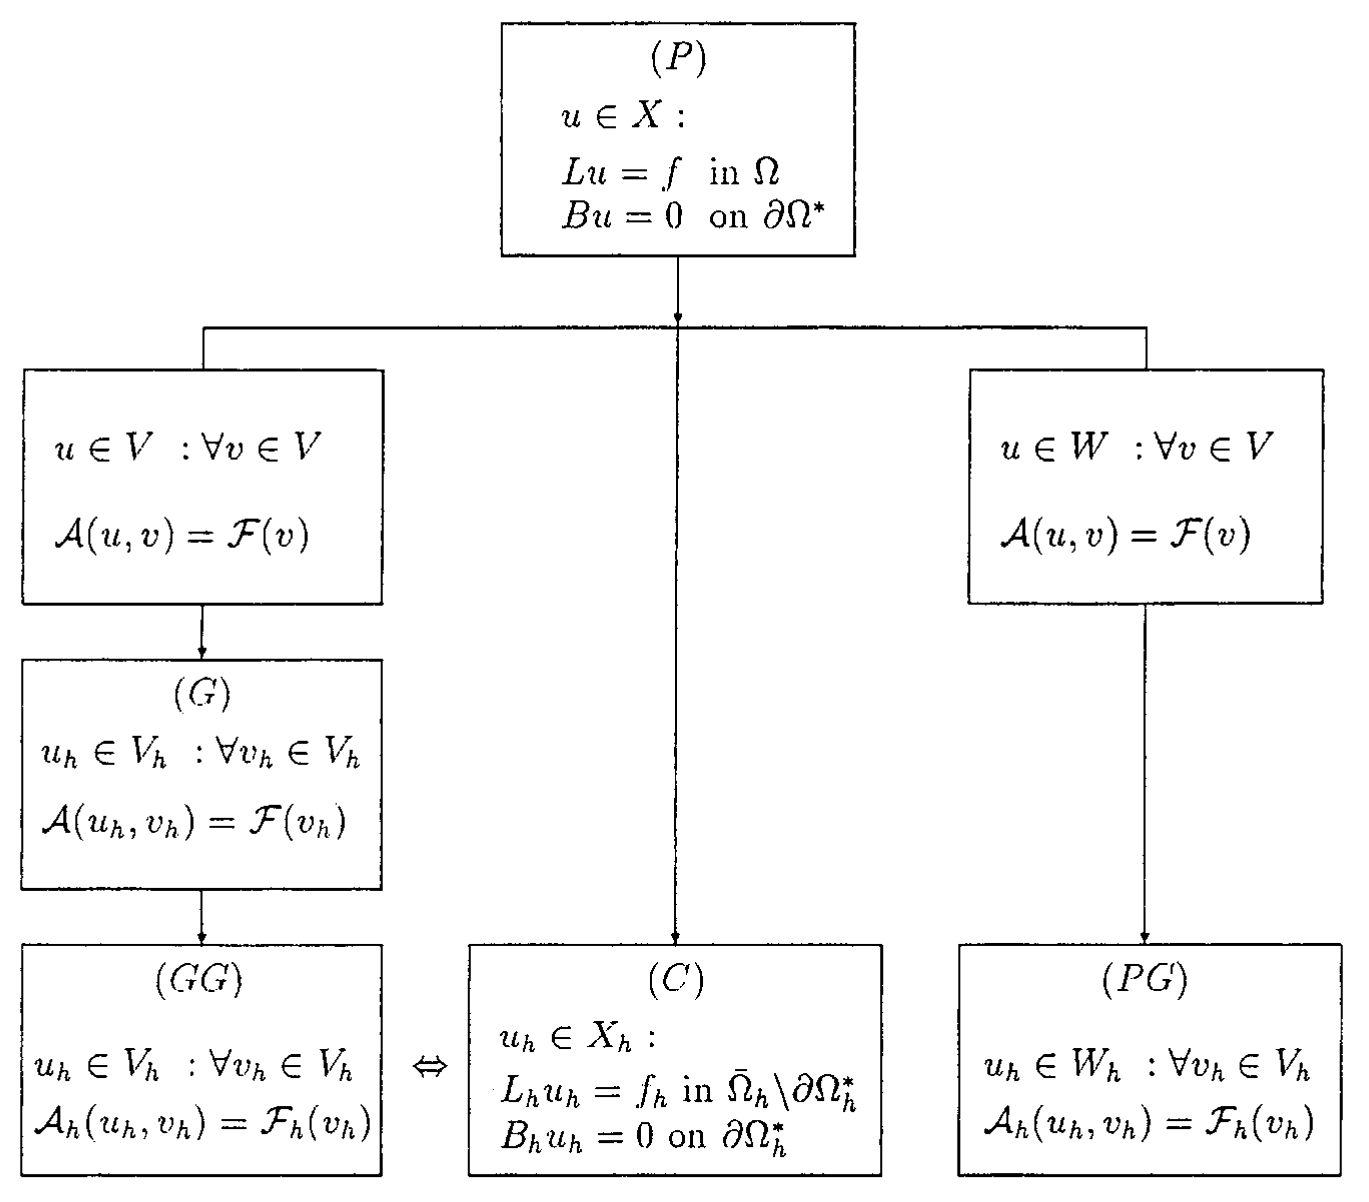
\includegraphics[width=.747\paperwidth]{images/fig-5-5-1.png}
  \caption{边值问题(P)的 Galerkin 逼近(G)、Petrov--Galerkin 逼近(PG)、广义 Galerkin 逼近(GG)和配置逼近(C)}\label{fig:5.5.1}
\end{figure}

\section{含时问题的时间推进方法}\label{sec:5.6}

本节讨论初边值问题的时间离散.这里仅作简要介绍,使读者对处理这一问题的几种方法有初步认识.本书\BookRef{part:3}{第三部分}将针对多类具体问题作详细讨论.

沿用第~\ref{sec:5.1}~节的抽象框架,现在定义下列问题：
\begin{equation}\label{eq:5.6.1}
  \begin{cases}
    \dfrac{\partial u}{\partial t}+Lu=f,&\text{在 }Q_T:=(0,T)\times\Omega\text{ 内},\\[2pt]
    Bu=0,&\text{在 }\Sigma_T^*:=(0,T)\times\partial\Omega^*\text{ 上},\\
    u=u_0,&\text{在 }\Omega\text{ 内,}t=0.
  \end{cases}
\end{equation}
\SourcePage{157}
这里 \(T>0\) 是给定的终止时刻,\(\partial/\partial t\) 表示对时间求导.未知量 \(u\) 和右端项 \(f\) 是 \(t\in(0,T)\) 与 \(\boldsymbol{x}\in\Omega\) 的函数,\(u_0=u_0(\boldsymbol{x})\) 是给定的初始数据.微分算子 \(L\) 和边界算子 \(B\) 现在可以依赖于 \(t\).

当 \(u\) 为向量值函数时,未必需要对它的每个分量作时间求导.下面介绍的 Stokes 问题便是一个例子.这类初边值问题称为\emph{微分代数方程}(见\BookCite{brenan-campbell-petzold1989}{Brenan、Campbell 和 Petzold(1989)}).

我们不讨论保证\eqref{eq:5.6.1}解的存在性和唯一性的一般假设.不过,可以假定上述问题能够写成弱形式.为此,假定存在三个 Hilbert 空间 \(V,W,H\),使得 \(W\) 和 \(V\) 都连续且稠密地嵌入 \(H\).除非另有说明,取 \(H=L^2(\Omega)\).\(H\) 中的内积记为 \((\cdot,\cdot)\).假定\SourcePage{158}\(u_0\in H\),\(f\in L^2(0,T;H)\).此外,假定存在 \(W\times V\) 上的连续双线性形式 \(\mathcal A(\cdot,\cdot)\).

\eqref{eq:5.6.1}的弱形式为：求 \(u\in L^2(0,T;W)\cap C^0([0,T];H)\)(这些空间的定义见第~\ref{sec:1.2}~节),使
\begin{equation}\label{eq:5.6.2}
  \frac{\mathrm d}{\mathrm dt}(u(t),v)+\mathcal A(u(t),v)
    =\mathcal F(t,v)\qquad\forall v\in V,
\end{equation}
并且 \(t=0\) 时 \(u=u_0\).对于微分代数系统,其中的时间导数及相应的时间连续性只涉及有时间导数的分量.右端项简记 \((f(t),v)\) 与非齐次边界条件可能产生的附加项之和.方程\eqref{eq:5.6.2}应按 \((0,T)\) 上的分布意义理解.在前述数据假设下,其中的运算都有意义.

下面给出三个例题,分别是第~\ref{sec:5.1}~节中三个例题的非定常版本.

\begin{example}[(热方程)]\label{ex:5.6.1}
考虑问题
\begin{equation}\label{eq:5.6.3}
  \begin{cases}
    \dfrac{\partial u}{\partial t}-\Delta u=f,&\text{在 }Q_T\text{ 内},\\[2pt]
    u=0,&\text{在 }\Sigma_T:=(0,T)\times\partial\Omega\text{ 上},\\
    u=u_0,&\text{在 }\Omega\text{ 内,}t=0.
  \end{cases}
\end{equation}
第~\BookRef{ch:11}{11}~章将详细讨论这个问题.它描述在外部热源 \(f\) 的作用下,\(\Omega\) 内各向同性均匀介质的温度 \(u\) 随时间的演化,其中 \(u_0\) 是初始温度.

其弱形式为：求 \(u\colon Q_T\to\mathbb R\),使 \(u(t,\cdot)\in H_0^1(\Omega)\),且
\begin{equation}\label{eq:5.6.4}
  \begin{aligned}
    &\int_\Omega\frac{\partial u}{\partial t}(t,\boldsymbol{x})v(\boldsymbol{x})\,\mathrm d\boldsymbol{x}
      +\int_\Omega\nabla u(t,\boldsymbol{x})\cdot\nabla v(\boldsymbol{x})\,\mathrm d\boldsymbol{x}\\
    &\qquad=\int_\Omega f(t,\boldsymbol{x})v(\boldsymbol{x})\,\mathrm d\boldsymbol{x}
      \qquad\forall v\in H_0^1(\Omega)
  \end{aligned}
\end{equation}
对几乎每个 \(t\in(0,T)\) 成立,并且 \(t=0\) 时 \(u=u_0\).因此,这是\eqref{eq:5.6.2}的一个特例,相应的记号见\eqref{eq:5.1.6}.
\end{example}

\begin{example}[(非定常 Stokes 问题)]\label{ex:5.6.2}
问题\eqref{eq:5.1.7}的含时版本为
\begin{equation}\label{eq:5.6.5}
  \begin{cases}
    \dfrac{\partial\boldsymbol{u}}{\partial t}-\nu\Delta\boldsymbol{u}+\nabla p
      =\boldsymbol{f},&\text{在 }Q_T\text{ 内},\\[2pt]
    \operatorname{div}\boldsymbol{u}=0,&\text{在 }Q_T\text{ 内},\\
    \boldsymbol{u}=\boldsymbol{0},&\text{在 }\Sigma_T\text{ 上},\\
    \boldsymbol{u}=\boldsymbol{u}_0,&\text{在 }\Omega\text{ 内,}t=0.
  \end{cases}
\end{equation}
\SourcePage{159}
这些方程描述 \(\Omega\) 内黏性不可压缩流体的非定常运动.这里假定流动缓慢,外力的体积密度为 \(\boldsymbol{f}\),初始速度为 \(\boldsymbol{u}_0\).第~\BookRef{ch:13}{13}~章将在含时 Navier--Stokes 方程的框架中推导这些方程.

\eqref{eq:5.6.5}的弱形式为：求 \(\boldsymbol{u}\colon Q_T\to\mathbb R^d\) 和 \(p\colon Q_T\to\mathbb R\),使得 \(\boldsymbol{u}(t,\cdot)\in(H_0^1(\Omega))^d\)、\(p(t,\cdot)\in L_0^2(\Omega)\),且
\begin{equation}\label{eq:5.6.6}
  \left\{
  \begin{aligned}
    &\int_\Omega \frac{\partial\boldsymbol{u}}{\partial t}(t,\boldsymbol{x})\cdot
           \boldsymbol{v}(\boldsymbol{x})\,\mathrm d\boldsymbol{x}
     +\nu\int_\Omega\nabla\boldsymbol{u}(t,\boldsymbol{x}):\nabla\boldsymbol{v}(\boldsymbol{x})\,\mathrm d\boldsymbol{x}\\
    &\qquad-\int_\Omega p(t,\boldsymbol{x})\operatorname{div}\boldsymbol{v}(\boldsymbol{x})\,\mathrm d\boldsymbol{x}\\
    &\qquad=\int_\Omega\boldsymbol{f}(t,\boldsymbol{x})\cdot\boldsymbol{v}(\boldsymbol{x})\,\mathrm d\boldsymbol{x}
             \qquad\forall\boldsymbol{v}\in(H_0^1(\Omega))^d,\\[3pt]
    &\int_\Omega q(\boldsymbol{x})\operatorname{div}\boldsymbol{u}(t,\boldsymbol{x})\,\mathrm d\boldsymbol{x}=0
             \qquad\forall q\in L_0^2(\Omega)
  \end{aligned}
  \right.
\end{equation}
对几乎每个 \(t\in(0,T)\) 成立,并且 \(t=0\) 时 \(\boldsymbol{u}=\boldsymbol{u}_0\).采用\eqref{eq:5.1.9}的记号,并只对速度分量求时间导数,又可将\eqref{eq:5.6.6}写成抽象形式\eqref{eq:5.6.2}.
\end{example}

\begin{example}[(线性输运问题)]\label{ex:5.6.3}
采用\eqref{eq:5.1.10}中的记号,输运方程的初边值问题为(另见第~\BookRef{ch:14}{14}~章)
\begin{equation}\label{eq:5.6.7}
  \begin{cases}
    \dfrac{\partial u}{\partial t}+\boldsymbol{a}\cdot\nabla u=f,
      &\text{在 }Q_T\text{ 内},\\[2pt]
    u=\varphi,&\text{在 }\Sigma_T^{\mathrm{in}}:=(0,T)\times\partial\Omega^{\mathrm{in}}\text{ 上},\\
    u=u_0,&\text{在 }\Omega\text{ 内,}t=0.
  \end{cases}
\end{equation}
这些方程描述量 \(u\) 的输运,其在任意点 \(\boldsymbol{x}\) 的传播速度由向量函数 \(\boldsymbol{a}\) 给出.为简便起见,可假定 \(\boldsymbol{a}\) 光滑且不依赖于 \(t\),这样流入边界 \(\partial\Omega^{\mathrm{in}}\) 不随时间变化.

\eqref{eq:5.6.7}的弱形式为：求 \(u\colon Q_T\to\mathbb R\),使 \(u(t,\cdot)\in L^2(\Omega)\),具有相应的流出迹,且
\begin{equation}\label{eq:5.6.8}
  \begin{aligned}
    &\int_\Omega\frac{\partial u}{\partial t}(t,\boldsymbol{x})v(\boldsymbol{x})\,\mathrm d\boldsymbol{x}
    -\int_\Omega u(t,\boldsymbol{x})\operatorname{div}(\boldsymbol{a}v)(\boldsymbol{x})\,\mathrm d\boldsymbol{x}\\
    &\quad+\int_{\partial\Omega\setminus\partial\Omega^{\mathrm{in}}}
      (\boldsymbol{a}\cdot\boldsymbol{n})(\boldsymbol{x})u(t,\boldsymbol{x})v(\boldsymbol{x})\,\mathrm d\gamma\\
    &=\int_\Omega f(t,\boldsymbol{x})v(\boldsymbol{x})\,\mathrm d\boldsymbol{x}
      -\int_{\partial\Omega^{\mathrm{in}}}(\boldsymbol{a}\cdot\boldsymbol{n})(\boldsymbol{x})
           \varphi(t,\boldsymbol{x})v(\boldsymbol{x})\,\mathrm d\gamma
     \qquad\forall v\in H^1(\Omega)
  \end{aligned}
\end{equation}
对几乎每个 \(t\in(0,T)\) 成立,并且 \(t=0\) 时 \(u=u_0\).由\eqref{eq:5.1.11}可见,这也是\eqref{eq:5.6.2}的一个例子.
\end{example}

\subsection{半离散逼近}\label{sec:5.6.1}
\SourcePage{160}

抽象问题\eqref{eq:5.6.2}需要对时间和空间两个变量作离散.

空间离散可以按定常问题的做法进行.例如,将\eqref{eq:5.2.3}的方法推广到\eqref{eq:5.6.2},便得到其 Galerkin 逼近.所得问题为：对每个 \(t\in[0,T]\),求 \(u_h(t,\cdot)\in V_h\subset V\),使得
\begin{equation}\label{eq:5.6.9}
  \frac{\mathrm d}{\mathrm dt}(u_h(t),v_h)+\mathcal A(u_h(t),v_h)
  =\mathcal F(t,v_h)\qquad\forall v_h\in V_h,\quad t\in(0,T),
\end{equation}
且 \(u_h(0)=u_{0,h}\),其中 \(u_{0,h}\) 是 \(V_h\) 中用来逼近初值 \(u_0\) 的适当元素.(通常取 \(u_0\) 的插值,或取它关于 \(L^2(\Omega)\) 内积或 \(V\) 内积的投影作为初值.)

类似地,也可引入基于 Petrov--Galerkin 法、广义 Galerkin 法或配置法的其他逼近.

问题\eqref{eq:5.6.9}常称为\eqref{eq:5.6.2}的\emph{半离散逼近},也称\emph{时间连续逼近}.令
\begin{equation}\label{eq:5.6.10}
  u_h(t,\boldsymbol{x})=\sum_{j=1}^{N_h}\xi_j(t)\varphi_j(\boldsymbol{x})\quad(t\ge0),
  \qquad
  u_{0,h}(\boldsymbol{x})=\sum_{j=1}^{N_h}\xi_{0,j}\varphi_j(\boldsymbol{x}),
\end{equation}
其中 \(\{\varphi_j\}\) 仍表示 \(V_h\) 的一组基.容易看出,\eqref{eq:5.6.9}给出关于未知向量 \(\boldsymbol{\xi}(t)\) 的常微分方程组：
\begin{equation}\label{eq:5.6.11}
  M\frac{\mathrm d\boldsymbol{\xi}(t)}{\mathrm dt}+A\boldsymbol{\xi}(t)
    =\boldsymbol{F}(t),\qquad \boldsymbol{\xi}(0)=\boldsymbol{\xi}_0.
\end{equation}
对每个 \(t\ge0\),\(\boldsymbol{\xi}(t)=(\xi_j(t))\),\(\boldsymbol{F}(t):=(\mathcal F(t,\varphi_i))\).此外,\(\boldsymbol{\xi}_0=(\xi_{0,j})\),且
\begin{equation}\label{eq:5.6.12}
  M_{ij}:=(\varphi_i,\varphi_j),\qquad
  A_{ij}:=\mathcal A(\varphi_j,\varphi_i),\qquad i,j=1,\ldots,N_h.
\end{equation}
刚度矩阵 \(A\) 与定常情形中引入的矩阵相同,见\eqref{eq:5.2.5}.若算子 \(L\) 不依赖于 \(t\),则 \(A\) 也不依赖于 \(t\).为便于论述,本节始终作此假设.对称正定矩阵 \(M\) 始终与 \(t\) 无关,称为\emph{质量矩阵}.对微分代数问题,相应质量矩阵在没有时间导数的分量上为零,因此不一定正定.

\subsection{全离散逼近}\label{sec:5.6.2}

\eqref{eq:5.6.9}的时间离散有多种做法.首先将时间区间 \([0,T]\) 分为 \(\mathcal N\) 个长度为 \(\Delta t=T/\mathcal N\) 的子区间 \([t_n,t_{n+1}]\),其中 \(t_0=0\),\(t_{\mathcal N}=T\).然后,在每个时刻 \(t_n\) 寻求 \(u(t_n)\) 的近似,以 \(u_h^n\) 记\SourcePage{161}相应的有限维函数.特别地,\(u_h^0\) 是 \(u_0\) 的一个适当近似.将问题\eqref{eq:5.6.9}完全离散化的经典做法,是用有限差分格式离散时间导数.这种格式用由 Taylor 展开公式得到的差商代替导数.下面通过常微分方程的 Cauchy 问题说明基本思想：
\begin{equation}\label{eq:5.6.13}
  \begin{cases}
    \dfrac{\mathrm dy}{\mathrm dt}(t)=\psi(t,y(t)),&0<t<T,\\
    y(0)=y_0,
  \end{cases}
\end{equation}
其中 \(\psi\colon[0,T]\times\mathbb R\to\mathbb R\) 是连续函数,且关于 \(y\) 满足对 \(t\in[0,T]\) 一致的 Lipschitz 条件.

在许多可能的有限差分格式中,先说明简单的 \(\theta\)-格式(\(0\le\theta\le1\)).按这一格式,上述问题由下式代替：
\begin{equation}\label{eq:5.6.14}
  \frac{y^{n+1}-y^n}{\Delta t}
    =\theta\psi(t_{n+1},y^{n+1})+(1-\theta)\psi(t_n,y^n),
\end{equation}
其中 \(n=0,\ldots,\mathcal N-1\),\(y^0=y_0\),\(y^n\) 逼近 \(y(t_n)\).

对\eqref{eq:5.6.9}应用 \(\theta\)-格式,得到
\begin{equation}\label{eq:5.6.15}
  \begin{aligned}
    &\frac1{\Delta t}(u_h^{n+1}-u_h^n,v_h)
     +\mathcal A(\theta u_h^{n+1}+(1-\theta)u_h^n,v_h)\\
    &\qquad=\theta\mathcal F(t_{n+1},v_h)+(1-\theta)\mathcal F(t_n,v_h)
            \qquad\forall v_h\in V_h,
  \end{aligned}
\end{equation}
其中 \(n=0,\ldots,\mathcal N-1\),\(u_h^0=u_{0,h}\).两个极端情形 \(\theta=0\) 和 \(\theta=1\) 分别给出熟知的前向 Euler 法和后向 Euler 法,它们关于时间步长 \(\Delta t\) 都是一阶精度.对应于 \(\theta=1/2\) 的格式称为 Crank--Nicolson 格式,在适当的光滑性条件下具有二阶精度.

两步法也能给出其他二阶格式.这类方法涉及 \(t_{n+1}\)、\(t_n\) 和 \(t_{n-1}\) 三个时刻.第一个例子是二阶 Adams--Bashforth 法：
\begin{equation}\label{eq:5.6.16}
  \frac{y^{n+1}-y^n}{\Delta t}
   =\frac32\psi(t_n,y^n)-\frac12\psi(t_{n-1},y^{n-1}),
   \qquad n=1,\ldots,\mathcal N-1.
\end{equation}
另一个例子是二阶后向差分法：
\begin{equation}\label{eq:5.6.17}
  \frac{3y^{n+1}-4y^n+y^{n-1}}{2\Delta t}=\psi(t_{n+1},y^{n+1}),
    \qquad n=1,\ldots,\mathcal N-1.
\end{equation}
两种格式都需要先求 \(y^1\),而且这一步的初始计算也必须具有二阶精度.将\eqref{eq:5.6.16}和\eqref{eq:5.6.17}用于\eqref{eq:5.6.9}的离散是直接的.

\SourcePage{162}
如果 \(u\) 及其直至 \(p+1\) 阶的时间导数连续,从形式上可以用 Taylor 公式达到 \(p\) 阶精度.

这里先指出,\eqref{eq:5.6.15}的代数形式为
\begin{equation}\label{eq:5.6.18}
  M\boldsymbol{\xi}^{n+1}+\theta\Delta t\,A\boldsymbol{\xi}^{n+1}=\boldsymbol{\eta}^{n+1},
    \qquad n=0,\ldots,\mathcal N-1,
\end{equation}
其中
\[
  \boldsymbol{\eta}^{n+1}:=\theta\Delta t\,\boldsymbol{F}(t_{n+1})
    +(1-\theta)\Delta t\,\boldsymbol{F}(t_n)
    +M\boldsymbol{\xi}^n+(\theta-1)\Delta t\,A\boldsymbol{\xi}^n,
\]
且 \(\boldsymbol{\xi}^0=\boldsymbol{\xi}_0\)(记号见\eqref{eq:5.6.10}–\eqref{eq:5.6.12}).如果先将有限差分格式用于\eqref{eq:5.6.2},再对所得的每一步定常问题作 Galerkin 空间逼近,也会得到相同的代数方程组.

当 \(\theta=0\) 时,除去对质量矩阵 \(M\) 的“求逆”,上述格式是显式的.如果 \(M\) 不是对角矩阵,常用质量集中把它变成对角形式,见第~\BookRef{sec:11.4}{11.4}~节.对于 \(\theta\) 的其他取值,\eqref{eq:5.6.18}都以隐式方式确定 \(\boldsymbol{\xi}^{n+1}\).类似地,\eqref{eq:5.6.16}是显式的,而\eqref{eq:5.6.17}是隐式的.

从计算的角度看,显式方法比隐式方法容易实现.其缺点是,显式方法一般只有\emph{条件稳定性}.对典型离散问题,时间步长 \(\Delta t\) 必须相对于 \(M^{-1}A\) 的最大特征值模的倒数足够小,因而也必须随空间尺度 \(h\) 取足够小的值.相反,某些隐式方法可以是\emph{无条件稳定的}.在这种情况下,\(\Delta t\) 的选取只由精度要求决定.

本书\BookRef{part:3}{第三部分}将针对所考虑的各类含时问题,具体说明这里提到的\emph{时间稳定性}概念.这里先作定性描述.对于 Cauchy 问题
\begin{equation}\label{eq:5.6.19}
  \begin{cases}
    \dfrac{\mathrm d\boldsymbol{\eta}}{\mathrm dt}(t)=B\boldsymbol{\eta}(t),
      &0<t<\infty,\\
    \boldsymbol{\eta}(0)=\boldsymbol{\eta}_0,
  \end{cases}
\end{equation}
其中 \(B\) 是给定的 \(m\) 阶矩阵,若存在与 \(\Delta t\) 无关的正常数 \(C,\lambda,\delta\),使得对所有 \(0<\Delta t\le\delta\),都有
\begin{equation}\label{eq:5.6.20}
  |\boldsymbol{\eta}^n|\le Ce^{\lambda t_n}|\boldsymbol{\eta}_0|,\qquad n\ge0,
\end{equation}
则称该方法稳定.这里 \(\boldsymbol{\eta}^n\) 是时刻 \(t_n=n\Delta t\) 的计算解,\(|\cdot|\) 是 \(\mathbb R^m\) 中的某个向量范数.

对于解 \(\boldsymbol{\eta}(t)\) 在所有 \(t>0\) 都有界的问题,\eqref{eq:5.6.20}允许的指数增长可能并不合适.这时,对时间离散方法提出\emph{绝对稳定性}要求更为恰当.这个概念定义如下.考虑标量\SourcePage{163}模型问题\eqref{eq:5.6.13},其中 \(\psi(t,y(t))=\mu y(t)\),\(\mu\in\mathbb C\).对给定的 \(\mu\Delta t\),若数值方法产生的近似解 \(y^n\) 在 \(n\to\infty\) 时趋于零,就称该方法对于这个 \(\mu\Delta t\) 是绝对稳定的.使方法绝对稳定的所有 \(\mu\Delta t\) 构成的集合称为\emph{绝对稳定域}.如果绝对稳定域包含 \(\{z\in\mathbb C\mid\operatorname{Re}z<0\}\),则称该方法为 \(A\)-稳定.容易证明,\(\theta\ge1/2\) 时,\(\theta\)-格式是 \(A\)-稳定的(例如,见\BookCite{lambert1991}{Lambert(1991)}第 244 页).

如果将\eqref{eq:5.6.19}换成半离散问题\eqref{eq:5.6.9},并取 \(\mathcal F(\cdot,\cdot)=0\)、\(T=\infty\),则当对所有 \(0<\Delta t\le\delta_h\) 都有
\begin{equation}\label{eq:5.6.21}
  \|u_h^n\|\le Ce^{\lambda t_n}\|u_h^0\|,\qquad n\ge0,
\end{equation}
便称时间推进方法关于 \(V_h\) 中的空间范数 \(\|\cdot\|\) 稳定.这里 \(C,\lambda,\delta_h\) 都与 \(\Delta t\) 无关,且 \(C,\lambda\) 也与 \(h\) 无关.若 \(\delta_h\) 具有与 \(h\) 无关的正下界,则这里称该方法为无条件稳定.否则,\(\delta_h\) 对 \(h\) 的函数依赖关系称为该数值方法的\emph{稳定性限制}.注意,对每个固定 \(h\),\(V_h\) 中的所有范数都等价,但等价常数一般不能对 \(h\) 一致选取.因此,\eqref{eq:5.6.21}可能只对适当选取的范数成立.

\section{分步法与算子分裂法}\label{sec:5.7}

分裂法是初边值问题时间离散的另一种工具.它也常用于求解形如\eqref{eq:5.1.1}的定常边值问题,把它的解看作相应含时问题\eqref{eq:5.6.1}的稳态.无论是哪种情形,其基本假设都是空间微分算子可以分裂成两个或更多结构较简单的部分之和.依次对这些部分作时间积分,便得到较简单的方程.

考虑形如
\begin{equation}\label{eq:5.7.1}
  \frac{\mathrm d\boldsymbol{\varphi}}{\mathrm dt}
    +\mathcal L\boldsymbol{\varphi}=\boldsymbol{\psi},\qquad t>0,
\end{equation}
的问题,其中 \(\mathcal L\) 是对给定微分算子作空间离散所产生的矩阵,已经计入边界条件；\(\boldsymbol{\psi}\) 是相应的右端项,\(\boldsymbol{\varphi}\) 是未知解.

对于 Galerkin 逼近,\(\mathcal L=M^{-1}A\),见\eqref{eq:5.6.11}.不过,也可以利用对称正定质量矩阵 \(M\) 的平方根作变量变换,取 \(\mathcal L=M^{-1/2}AM^{-1/2}\).在后一情形下,若 \(A\) 对称,则 \(\mathcal L\) 也对称.

对于谱配置逼近,质量矩阵 \(M\) 是对角矩阵,甚至可以是单位矩阵 \(I\)(见第~\BookRef{sec:11.4}{11.4}~节).在后一种情形下,直接取 \(\mathcal L=A\) 即可.

\SourcePage{164}
为简便起见,假设 \(\mathcal L\) 只是两个部分之和：
\begin{equation}\label{eq:5.7.2}
  \mathcal L=\mathcal L_1+\mathcal L_2,
\end{equation}
每个部分都与时间变量无关.现有分裂法理论大多只适用于下列情形：
\begin{equation}\label{eq:5.7.3}
  \text{\(\mathcal L_1\) 和 \(\mathcal L_2\) 都是正定矩阵(或半正定矩阵).}
\end{equation}
不过,分裂法所适用的问题远比这一类广泛.

还要指出,分裂经常直接作用于微分算子本身,在离散之前写成
\begin{equation}\label{eq:5.7.4}
  L=L_1+L_2,
\end{equation}
与在代数层面作\eqref{eq:5.7.2}的做法有所不同.直接分裂微分算子格外有吸引力,因为往往可以从物理角度出发,使 \(L_1\) 和 \(L_2\) 各有明确的物理含义,例如分别表示扩散和输运过程.不过,内在的数学困难是,\eqref{eq:5.7.4}通常也要求分拆边界条件,从而为 \(L_1\) 和 \(L_2\) 配上相容的边界数据.第~\BookRef{ch:12}{12}~章和第~\BookRef{ch:13}{13}~章将回到这个问题,讨论用于对流--扩散方程和 Navier--Stokes 方程组的若干分步法.

这里仍讨论\eqref{eq:5.7.1}–\eqref{eq:5.7.2}的情形.照例令 \(t_0=0\),并令 \(t_{n+1}=t_n+\Delta t\)(\(n\ge0\)).同时,取 \(\boldsymbol{\varphi}^0\) 为初始数据 \(u_0\) 的适当近似.

先考虑 \emph{Yanenko 分裂}：
\begin{equation}\label{eq:5.7.5}
  \begin{cases}
    \dfrac{\boldsymbol{\varphi}^{n+1/2}-\boldsymbol{\varphi}^n}{\tau}
     +\mathcal L_1\boldsymbol{\varphi}^{n+1/2}=\boldsymbol{0},\\[4pt]
    \dfrac{\boldsymbol{\varphi}^{n+1}-\boldsymbol{\varphi}^{n+1/2}}{\tau}
     +\mathcal L_2\boldsymbol{\varphi}^{n+1}=\boldsymbol{\psi}^n,
  \end{cases}
\end{equation}
其中 \(n\ge0\),\(\tau=\Delta t\).这一方法产生两个隐式问题.若问题数据足够光滑,它关于 \(\Delta t\) 是一阶精度的.事实上,消去 \(\boldsymbol{\varphi}^{n+1/2}\) 后得到
\[
  \frac{\boldsymbol{\varphi}^{n+1}-\boldsymbol{\varphi}^n}{\Delta t}
  +\mathcal L\boldsymbol{\varphi}^{n+1}
   =\boldsymbol{\psi}^n+\Delta t\,\mathcal L_1
          (\boldsymbol{\psi}^n-\mathcal L_2\boldsymbol{\varphi}^{n+1}).
\]
此外,在条件\eqref{eq:5.7.3}下,分裂格式\eqref{eq:5.7.5}无条件稳定(\BookCite{marchuk1990}{Marchuk(1990)},第 232 页).

若 \(L\) 是二维负 Laplace 算子,而 \(\mathcal L_i\) 是 \(-\partial^2/\partial x_i^2\)(\(i=1,2\))的离散对应,则上述分裂格式给出经典的\emph{交替方向法}.其对三维负 Laplace 算子的三阶段推广\SourcePage{165}可直接写出.

\emph{预测--校正格式}是下列三阶段方法：
\begin{equation}\label{eq:5.7.6}
  \begin{cases}
    \dfrac{\boldsymbol{\varphi}^{n+1/4}-\boldsymbol{\varphi}^n}{\tau}
      +\mathcal L_1\boldsymbol{\varphi}^{n+1/4}=\boldsymbol{\psi}^{n+1/2},\\[4pt]
    \dfrac{\boldsymbol{\varphi}^{n+1/2}-\boldsymbol{\varphi}^{n+1/4}}{\tau}
      +\mathcal L_2\boldsymbol{\varphi}^{n+1/2}=\boldsymbol{0},\\[4pt]
    \dfrac{\boldsymbol{\varphi}^{n+1}-\boldsymbol{\varphi}^n}{2\tau}
      +\mathcal L\boldsymbol{\varphi}^{n+1/2}=\boldsymbol{\psi}^{n+1/2},
  \end{cases}
\end{equation}
其中 \(\tau=\Delta t/2\),\(\boldsymbol{\psi}^{n+1/2}\) 是右端项在中间时刻 \(t_{n+1/2}=t_n+\Delta t/2\) 的取值.预测步骤通过两个隐式方程给出 \(\boldsymbol{\varphi}^{n+1/2}\),它是 \(t_{n+1/2}\) 时刻解的一阶近似；二阶校正步骤再显式给出新解 \(\boldsymbol{\varphi}^{n+1}\).

这一方法在形式上具有二阶精度.事实上,消去 \(\boldsymbol{\varphi}^{n+1/4}\) 可得
\[
  \frac{\boldsymbol{\varphi}^{n+1/2}-\boldsymbol{\varphi}^n}{\Delta t}
  +\frac12\mathcal L\boldsymbol{\varphi}^{n+1/2}
  +\frac{\Delta t}4\mathcal L_1\mathcal L_2\boldsymbol{\varphi}^{n+1/2}
    =\frac12\boldsymbol{\psi}^{n+1/2}.
\]
利用\eqref{eq:5.7.6}的第三式表示 \(\mathcal L\boldsymbol{\varphi}^{n+1/2}\),得到
\[
  \boldsymbol{\varphi}^{n+1/2}
   =\frac12(\boldsymbol{\varphi}^{n+1}+\boldsymbol{\varphi}^n)
      -\frac{(\Delta t)^2}4\mathcal L_1\mathcal L_2\boldsymbol{\varphi}^{n+1/2}.
\]
因此,有
\[
  \frac{\boldsymbol{\varphi}^{n+1}-\boldsymbol{\varphi}^n}{\Delta t}
   +\mathcal L\left(\frac{\boldsymbol{\varphi}^{n+1}+\boldsymbol{\varphi}^n}{2}\right)
   =\boldsymbol{\psi}^{n+1/2}
      +\frac{(\Delta t)^2}4\mathcal L\mathcal L_1\mathcal L_2\boldsymbol{\varphi}^{n+1/2}.
\]
由于
\[
  \begin{aligned}
    \boldsymbol{\varphi}^{n+1/2}
    &=\left(I+\frac{\Delta t}2\mathcal L_2\right)^{-1}
      \left(I+\frac{\Delta t}2\mathcal L_1\right)^{-1}
      \left(\boldsymbol{\varphi}^n+\frac{\Delta t}2\boldsymbol{\psi}^{n+1/2}\right)\\
    &=\boldsymbol{\varphi}^n+O(\Delta t),
  \end{aligned}
\]
最终有
\[
  \begin{aligned}
    &\frac{\boldsymbol{\varphi}^{n+1}-\boldsymbol{\varphi}^n}{\Delta t}
       +\mathcal L\left(\frac{\boldsymbol{\varphi}^{n+1}+\boldsymbol{\varphi}^n}{2}\right)\\
    &\qquad=\boldsymbol{\psi}^{n+1/2}
       +\frac{(\Delta t)^2}4\mathcal L\mathcal L_1\mathcal L_2\boldsymbol{\varphi}^n
       +O((\Delta t)^3).
  \end{aligned}
\]
这与 Crank--Nicolson 格式相差 \(O((\Delta t)^2)\).若 \(\mathcal L_1\) 与 \(\mathcal L_2\) 可交换,确实可写为
\[
  \begin{aligned}
    &\frac{\boldsymbol{\varphi}^{n+1}-\boldsymbol{\varphi}^n}{\Delta t}
       +\mathcal L\left(\frac{\boldsymbol{\varphi}^{n+1}+\boldsymbol{\varphi}^n}{2}\right)\\
    &\qquad=\boldsymbol{\psi}^{n+1/2}
       +\frac{(\Delta t)^2}4\mathcal L_1\mathcal L_2
        \left(\boldsymbol{\psi}^{n+1/2}
           -\frac{\boldsymbol{\varphi}^{n+1}-\boldsymbol{\varphi}^n}{\Delta t}\right).
  \end{aligned}
\]

\SourcePage{166}
只要\eqref{eq:5.7.3}成立,预测--校正格式就无条件稳定,即使校正步骤单独考虑时可能不稳定.参见\BookCite{marchuk1990}{Marchuk(1990,第 271 页)}.

Peaceman 和 Rachford 的分裂法为
\begin{equation}\label{eq:5.7.7}
  \begin{cases}
    \dfrac{\boldsymbol{\varphi}^{n+1/2}-\boldsymbol{\varphi}^n}{\tau}
      +\mathcal L_1\boldsymbol{\varphi}^{n+1/2}=\boldsymbol{\psi}^{n+1/2}-\mathcal L_2\boldsymbol{\varphi}^n,\\[4pt]
    \dfrac{\boldsymbol{\varphi}^{n+1}-\boldsymbol{\varphi}^{n+1/2}}{\tau}
      +\mathcal L_2\boldsymbol{\varphi}^{n+1}=\boldsymbol{\psi}^{n+1/2}-\mathcal L_1\boldsymbol{\varphi}^{n+1/2},
  \end{cases}
\end{equation}
其中 \(\tau=\Delta t/2\).这一方法具有二阶精度,见下文\eqref{eq:5.7.10}.在二维情形下,若 \(\mathcal L_i\) 是 \(-\partial^2/\partial x_i^2\) 的适当逼近,则这一格式无条件稳定.推广到三维后,这一性质便不再成立.

Douglas 和 Rachford 的方法与此类似：
\begin{equation}\label{eq:5.7.8}
  \begin{cases}
    \dfrac{\boldsymbol{\varphi}^{n+1/2}-\boldsymbol{\varphi}^n}{\tau}
      +\mathcal L_1\boldsymbol{\varphi}^{n+1/2}=\boldsymbol{\psi}^n-\mathcal L_2\boldsymbol{\varphi}^n,\\[4pt]
    \dfrac{\boldsymbol{\varphi}^{n+1}-\boldsymbol{\varphi}^{n+1/2}}{\tau}
      +\mathcal L_2\boldsymbol{\varphi}^{n+1}=\mathcal L_2\boldsymbol{\varphi}^n,
  \end{cases}
\end{equation}
其中 \(\tau=\Delta t\).这一格式只有一阶精度,见下文\eqref{eq:5.7.10}.但即使推广到 \(\mathcal L=\mathcal L_1+\mathcal L_2+\mathcal L_3\),且 \(\mathcal L_i\) 是 \(-\partial^2/\partial x_i^2\) 的适当逼近,它仍是无条件稳定的(见\BookCite{marchuk1990}{Marchuk(1990)}第 277–279 页).

\emph{Il’in 法}给出了同时推广\eqref{eq:5.7.7}和\eqref{eq:5.7.8}的分裂格式：
\begin{equation}\label{eq:5.7.9}
  \begin{cases}
    \dfrac{\boldsymbol{\varphi}^{n+1/2}-\boldsymbol{\varphi}^n}{\tau}
      +\mathcal L_1\boldsymbol{\varphi}^{n+1/2}=\boldsymbol{\psi}^{n+1/2}-\mathcal L_2\boldsymbol{\varphi}^n,\\[4pt]
    \dfrac{\boldsymbol{\varphi}^{n+1}-\boldsymbol{\varphi}^{n+1/2}}{\tau}
      +\mathcal L_2(\boldsymbol{\varphi}^{n+1}-\boldsymbol{\varphi}^n)
      =\rho\dfrac{\boldsymbol{\varphi}^{n+1/2}-\boldsymbol{\varphi}^n}{\tau},
  \end{cases}
\end{equation}
其中 \(\tau=\Delta t/(1+\rho)\),而 \(\rho\in(-1,1]\) 是一个参数.当 \(\rho=0\) 和 \(\rho=1\) 时,\eqref{eq:5.7.9}分别成为\eqref{eq:5.7.8}(右端用 \(\boldsymbol{\psi}^{n+1/2}\) 代替 \(\boldsymbol{\psi}^n\))和\eqref{eq:5.7.7}.

消去 \(\boldsymbol{\varphi}^{n+1/2}\),得到
\begin{equation}\label{eq:5.7.10}
  \begin{aligned}
    &\frac{\boldsymbol{\varphi}^{n+1}-\boldsymbol{\varphi}^n}{\Delta t}
      +\mathcal L\left(\frac{\boldsymbol{\varphi}^{n+1}}{1+\rho}
                   +\frac{\rho\boldsymbol{\varphi}^n}{1+\rho}\right)\\
    &\qquad=\boldsymbol{\psi}^{n+1/2}
      -\frac{(\Delta t)^2}{(1+\rho)^2}\mathcal L_1\mathcal L_2
       \left(\frac{\boldsymbol{\varphi}^{n+1}-\boldsymbol{\varphi}^n}{\Delta t}\right).
  \end{aligned}
\end{equation}
因此,\(\rho=1\) 时这一格式具有二阶精度,此时它与 Peaceman--Rachford 格式一致；其余情形均为一阶精度.此外,当 \(\mathcal L_i\) 满足\eqref{eq:5.7.3}时,它对任意 \(\rho\in(-1,1]\) 都无条件稳定(见\BookCite{yanenko1971}{Yanenko(1971)}第 65 页和\BookCite{marchuk1990}{Marchuk(1990)}第 291 页).

\SourcePage{167}
一种三阶段分裂格式是所谓的 \(\vartheta\)-法(或 Strang 法,见\BookCite{strang1968}{Strang(1968)})：
\begin{equation}\label{eq:5.7.11}
  \begin{cases}
    \dfrac{\boldsymbol{\varphi}^{n+\vartheta}-\boldsymbol{\varphi}^n}{\vartheta\tau}
      +\mathcal L_1\boldsymbol{\varphi}^{n+\vartheta}=\boldsymbol{\psi}^n-\mathcal L_2\boldsymbol{\varphi}^n,\\[4pt]
    \dfrac{\boldsymbol{\varphi}^{n+1-\vartheta}-\boldsymbol{\varphi}^{n+\vartheta}}{(1-2\vartheta)\tau}
      +\mathcal L_2\boldsymbol{\varphi}^{n+1-\vartheta}
       =\boldsymbol{\psi}^{n+1-\vartheta}-\mathcal L_1\boldsymbol{\varphi}^{n+\vartheta},\\[4pt]
    \dfrac{\boldsymbol{\varphi}^{n+1}-\boldsymbol{\varphi}^{n+1-\vartheta}}{\vartheta\tau}
      +\mathcal L_1\boldsymbol{\varphi}^{n+1}
       =\boldsymbol{\psi}^{n+1-\vartheta}-\mathcal L_2\boldsymbol{\varphi}^{n+1-\vartheta},
  \end{cases}
\end{equation}
其中 \(\tau=\Delta t\),\(\vartheta\) 是严格小于 \(1/2\) 的正实数.取 \(\vartheta=1-\sqrt2/2\) 时,该格式具有二阶精度,否则为一阶精度.另一方面,本书写作时还没有完整的稳定性分析.其他说明见\BookCite{glowinski-letallec1989}{Glowinski 和 Le Tallec(1989)}.

如前所述,若 \(\boldsymbol{\psi}\) 不依赖于 \(t\),以上分裂法除 Yanenko 格式和预测--校正格式外,都可用于求解定常问题 \(\mathcal L\boldsymbol{\chi}=\boldsymbol{\psi}\).事实上,只要 \(\boldsymbol{\varphi}^n\) 收敛,设 \(\boldsymbol{\varphi}^n\to\boldsymbol{\varphi}^\infty\),就有 \(\boldsymbol{\varphi}^\infty=\boldsymbol{\chi}\)(当定常问题的解唯一时).在这类应用中,应把 \(\tau\) 视为加速收敛的参数,其选取不再由物理时间步长决定.关于这一点,另见第~\ref{sec:2.3.5}~节.

文献中还有许多其他分裂法,有兴趣的读者可参见\BookCite{yanenko1971}{Yanenko(1971)}和\BookCite{marchuk1990}{Marchuk(1990)}.这些方法常针对具体方程构造,以反映整个问题中性质各异的物理过程.第~\BookRef{ch:12}{12}~章和第~\BookRef{ch:13}{13}~章将给出一些例子.

\begin{note}\NumberedNote{note:5.7.1}{\heiti(关于术语)}
在文献中,“算子分裂”与“分步”经常互作同义词.为求精确,宜用“算子分裂”指给定微分算子的分解\eqref{eq:5.7.4},或相应矩阵的分解\eqref{eq:5.7.2}；“分步”则指在已选定的算子分裂基础上,把问题从 \(t_n\) 推进到 \(t_{n+1}\) 的方法,例如 Douglas--Rachford 法和 Peaceman--Rachford 法.因此,同一种算子分裂可以配合多种分步格式.类似地,同一种分步格式可以用于不同的算子分裂,例如既用于 \(L=L_1+L_2\),也用于 \(L=L_3+L_4\),其中 \(L_1\ne L_3\) 且 \(L_1\ne L_4\).\hfill\(\square\)
\end{note}

\section{补充说明}\label{sec:5.8}
\SourcePage{168}

本章无意穷尽所有数值方法,因此还有许多方法未曾讨论.

\emph{有限差分法}或许是最常用的空间离散工具.第~\BookRef{ch:8}{8}~章和第~\BookRef{ch:14}{14}~章将广泛讨论这一方法.要系统了解这一主题,可参阅大量现有文献.这里特别提到\BookCite{forsythe-wasow1960}{Forsythe 和 Wasow(1960)}、\BookCite{godunov-ryabenkii1987}{Godunov 和 Ryaben’kii(1987)}、\BookCite{richtmyer-morton1967}{Richtmyer 和 Morton(1967)}以及\BookCite{samarskii-andreev1978}{Samarskiĭ 和 Andreev(1978)}的经典专著,也可参见较新的\BookCite{heinrich1987}{Heinrich(1987)}、\BookCite{strikwerda1989}{Strikwerda(1989)}及其所引文献.

某些椭圆型边值问题,例如外部区域上的 Laplace 方程,会导出积分方程.逼近这类积分方程的一种很成功的方法是所谓的\emph{边界元法}.借助微分算子的基本解,把问题改写为区域边界上的积分方程,再在适当的有限维分片多项式子空间中寻求近似解.有兴趣的读者可参见\BookCite{wendland1979}{Wendland(1979)}及\BookCite{brebbia-telles-wrobel1984}{Brebbia、Telles 和 Wrobel(1984)}.关于这一主题,较新的专著有\BookCite{chen-zhou1992}{Chen 和 Zhou(1992)},也可参见其中引用的文献.

\emph{有限体积法}的离散源于以积分形式表示的守恒律.因此,它主要用于计算流体动力学.第~\BookRef{sec:14.6}{14.6}~节将简要介绍这一方法,并给出多篇参考文献.

特殊的时空积分技术包括所谓的\emph{间断 Galerkin 法}和 \emph{Taylor--Galerkin 法}.这两种方法都已应用于双曲型初边值问题,将在第~\BookRef{sec:14.3.3}{14.3.3}~节和第~\BookRef{sec:14.3.4}{14.3.4}~节介绍.间断 Galerkin 法也可用于逼近抛物型问题,见第~\BookRef{sec:11.3.1}{11.3.1}~节和第~\BookRef{sec:12.3}{12.3}~节.

第~\ref{sec:5.2}~节至第~\ref{sec:5.5}~节给出的所有收敛结论,都基于所谓的\emph{先验误差分析}.只要数值方法稳定,且与原边值问题相容,它便收敛.这是 Lax--Richtmyer 等价定理所体现的原理在此处的推广.该定理断言,对于线性适定初值问题,一个相容的差分格式收敛当且仅当它稳定.随具体情形而异,对于 Galerkin 逼近,相容性假设可以采用\eqref{eq:5.2.2}和\eqref{eq:5.2.8}的形式；对于 Petrov--Galerkin 法和广义 Galerkin 法,则可由\eqref{eq:5.2.2}以及近似形式 \(\mathcal A_h\) 和 \(\mathcal F_h\) 在 \(h\to0\) 时分别以适当方式趋于 \(\mathcal A\) 和 \(\mathcal F\) 来表达.在后面各章中会看到,利用这样的分析可以推出误差估计,表明误差的某个适当范数可以用常数 \(C_{\mathrm{pr}}\) 乘以 \(h\) 的某个幂来控制.

\SourcePage{169}
一种互补的方法是所谓的\emph{后验误差分析}.它只能在实际完成一次计算之后使用,也就是“后验”地使用.其目的是给出误差上界,写成可以较精确估计的常数 \(C_{\mathrm{post}}\) 与易于计算的原问题残差的乘积.后验分析表明,若数值方法稳定,并且它给出的解的残差趋于零,则该格式收敛.后验分析对某些复杂问题尤其有用,例如非线性问题.在这些问题中,为使误差低于所要求的容差,往往要在整个求解过程中进行某种自适应调整.

建立后验误差分析,或提出和分析自适应方法,超出了本书的范围.不过,这是一个很值得关注的研究方向.有关参考资料,例如可见\BookCite{eriksson-estep-hansbo-johnson1995}{Eriksson、Estep、Hansbo 和 Johnson(1995)}的专著.此外,还可参阅较早的论文：\BookCite{babuska1976}{Babuška(1976)}、\BookCite{babuska-rheinboldt1978a}{Babuška 和 Rheinboldt(1978a}、\BookCite{babuska-rheinboldt1978b}{1978b)}、\BookCite{bank-wieser1985}{Bank 和 Wieser(1985)}、\BookCite{babuska-miller1987}{Babuška 和 Miller(1987)}、\BookCite{zienkiewicz-zhu1987}{Zienkiewicz 和 Zhu(1987)}、\BookCite{ainsworth-zhu-craig-zienkiewicz1989}{Ainsworth、Zhu、Craig 和 Zienkiewicz(1989)}、\BookCite{verfurth1989}{Verfürth(1989)}、\BookCite{ainsworth-oden1993}{Ainsworth 和 Oden(1993)},以及由\BookCite{babuska-chandra-flaherty1983}{Babuška、Chandra 和 Flaherty(1983)}、\BookCite{babuska-zienkiewicz-gago-arantes1986}{Babuška、Zienkiewicz、Gago 和 de Arantes e Oliveira(1986)}、\BookCite{oden1990}{Oden(1990)}以及\BookCite{demkowicz-oden-babuska1992}{Demkowicz、Oden 和 Babuška(1992)}编辑的著作.

\BookCite{johnson1987}{Johnson(1987)}第 4.6 节简要介绍了基于先验误差估计的自适应方法.
